\documentclass[tcc,capa]{texufpel}

\usepackage[utf8]{inputenc} % acentuacao
\usepackage{graphicx} % para inserir figuras
\usepackage[T1]{fontenc}
\usepackage{hyperref}
\usepackage{subcaption}
\usepackage{float}
\usepackage{microtype}
\usepackage{tabularx}
\setlength{\emergencystretch}{3em}
\hypersetup{
    hidelinks, % Remove coloração e caixas
    unicode=true,   %Permite acentuação no bookmark
    linktoc=all %Habilita link no nome e página do sumário
}



\unidade{Centro de Desenvolvimento Tecnológico}
\curso{Engenharia de Computação}
\nomecurso{Bacharelado em Engenharia de Computação}
\titulocurso{Bacharel em Engenharia de Computação}

\unidadeeng{Technology Development Center}
\cursoeng{Computer Science}


\title{VideoLearnAI: LLM Powered Web Application para aprendizagem ativa com vídeos do Youtube}

\author{Weitgenant}{Kevin Castro}
\advisor[Prof.~Dr.]{Primo}{Tiago}
\coadvisor[Prof.~Dr.]{Aguiar}{Marilton Sanchotene de}

%Palavras-chave em PT_BR
%use letras minúsculas seguidas por ;
%a última terminada por .
\keyword{aprendizagem ativa;}
\keyword{large language models;}
\keyword{processamento de linguagem natural;}
\keyword{educação online.}

%Palavras-chave em EN_US
\keywordeng{active learning;}
\keywordeng{large language models;}
\keywordeng{natural language processing;}
\keywordeng{online education.}

% Adicionar no preâmbulo, antes de \begin{document}
\tolerance=1500
\pretolerance=250
\hbadness=1500

% Redefine o ambiente englishabstract para usar ABSTRACT como título
\makeatletter
\renewenvironment{englishabstract}[1]{%
  \if@openright\cleardoublepage\else\clearpage\fi%
  \gdef\@englishtitle{{#1}}%
  \iflanguage{english}{
    \begin{otherlanguage}{brazilian}
    }{
      \begin{otherlanguage}{english}
      }

      \chapter*{ABSTRACT}
      \noindent{\MakeUppercase{\@authoralast},
        \@authorafirst. \textbf{\@englishtitle}. \advisorname: \@advisorafirst\ \@advisoralast. \@publyear. \pageref{LastPage}~f. \@tipodocumento,
        \universidadename, \@city, \@publyear.}\\~\\
    }{
      \par\vfill
      \noindent Keywords: \@abstractkweng
    \end{otherlanguage}
}
\makeatother

% Ou, para ignorar completamente os avisos de underfull/overfull hbox
% \hfuzz=\maxdimen
% \vfuzz=\maxdimen
% \hbadness=10000
% \vbadness=10000

\begin{document}

%\renewcommand{\advisorname}{Orientadora}           %descomente caso tenhas orientadora
%\renewcommand{\coadvisorname}{Coorientadora}      %descomente caso tenhas coorientadora

\maketitle 

\sloppy

\fichacatalografica

%\folhadeaprovacao

%Composição da Banca Examinadora
\begin{aprovacao}{16 de março de 2025} %data da banca por extenso
\noindent Prof. Dr. Marilton Sanchotene de Aguiar (orientador)\\
Doutor em Computação pela Universidade Federal do Rio Grande do Sul.\\[1cm]

\noindent Prof. Dr. Paulo Roberto Ferreira Jr.\\
Doutor em Computação pela Universidade Federal do Rio Grande do Sul.\\[1cm]

\noindent Prof. Dr. Ricardo Matsumura Araujo\\
Doutor em Computação pela Universidade Federal do Rio Grande do Sul.\\[1cm]

\noindent Prof. Dr. Luciano da Silva Pinto\\
Doutor em Biotecnologia pela Universidade Federal de Pelotas.
\end{aprovacao}

%Opcional
\begin{dedicatoria}
  Dedico\ldots 
\end{dedicatoria}

%Opcional
\begin{agradecimentos}
  Agradeço\ldots 
\end{agradecimentos}

%Opcional
\begin{epigrafe}
  What would life be if we had no courage to attempt anything?\\
  {\sc --- Vincent van Gogh}
\end{epigrafe}


%Resumo em Portugues (no maximo 500 palavras)
\begin{abstract}
  Este trabalho apresenta o desenvolvimento de um Software como Serviço (SaaS) potencializado por Large Language Models (LLMs) para transformar o consumo passivo de vídeos educacionais em experiências de aprendizagem ativa. Apesar da abundância de conteúdo educacional de alta qualidade disponível online, em geral, as pessoas assistem a esses vídeos de forma passiva, o que limita a compreensão e a retenção do conhecimento, uma vez que a aprendizagem mais efetiva ocorre através do engajamento ativo com o material. Para resolver este problema, o sistema VideoLearnAI implementa cinco funcionalidades principais: melhoria automática da legibilidade de legendas utilizando o modelo SaT (Segment Any Text), geração de capítulos para navegação estruturada, transcrição sincronizada de alta qualidade, quizzes interativos personalizáveis e um sistema de bate-papo contextual baseado no conteúdo do vídeo. A implementação focou em escalabilidade e desempenho, utilizando processamento GPU e técnicas modernas de desenvolvimento de software. Os resultados demonstram o potencial da solução para tornar vídeos educacionais mais engajantes e eficazes, criando experiências de aprendizagem personalizadas e interativas que promovem maior retenção de conhecimento e compreensão mais profunda do conteúdo.
  
\end{abstract}
  
%Resumo em Inglês (no maximo 500 palavras)
\begin{englishabstract}{VideoLearnAI: LLM-Powered Web Application for Active Learning with YouTube Videos}
  This work presents the development of an LLM-powered Software as a Service (SaaS) that transforms passive video consumption into active learning experiences. Despite the abundance of high-quality educational content available online, people generally watch these videos passively, which limits comprehension and knowledge retention, as more effective learning occurs through active engagement with the material. To address this challenge, the VideoLearnAI system implements five main functionalities: automatic subtitle readability improvement using the SaT (Segment Any Text) model, chapter generation for structured navigation, high-quality synchronized transcription, customizable interactive quizzes, and a contextual chat system based on video content. The implementation focused on scalability and performance, utilizing GPU processing and modern software development techniques. The results demonstrate the solution's potential to make educational videos more engaging and effective, creating personalized and interactive learning experiences that promote greater knowledge retention and deeper understanding of content.
  
\end{englishabstract}

%Lista de Figuras
\listoffigures

%Lista de Tabelas
\listoftables

%lista de abreviaturas e siglas
\begin{listofabbrv}{SaaS}%coloque aqui a maior sigla para ajustar a distância
        \item[SaaS] Software as a Service
        \item[API] Application Programming Interface
        \item[ASR] Automatic Speech Recognition
        \item[GPU] Graphics Processing Unit
        \item[IDE] Integrated Development Environment
        \item[JSON] JavaScript Object Notation
        \item[JWT] JSON Web Token
        \item[LLM] Large Language Model
        \item[ORM] Object-Relational Mapping
        \item[RAG] Retrieval-Augmented Generation
        \item[REST] Representational State Transfer
        \item[SaT] Segment Any Text
        \item[SSE] Server-Sent Events
        \item[UI] User Interface
        \item[UX] User Experience
\end{listofabbrv}

%Sumario
\tableofcontents

\chapter{Introdução}
Nos últimos anos, o consumo de conteúdo educacional em vídeo tem crescido exponencialmente, impulsionado por plataformas como YouTube\footnote{\url{https://www.youtube.com}}, Coursera\footnote{\url{https://www.coursera.org}} e Udemy\footnote{\url{https://www.udemy.com}}. Hoje, é possível encontrar aulas completas de universidades de altíssimo nível, como MIT, Harvard e Stanford, gratuitamente disponíveis online. No entanto, apesar da abundância de material de qualidade, muitos usuários enfrentam dificuldades em absorver e reter conhecimento de forma eficiente. A maioria das pessoas consome esses conteúdos de maneira passiva, apenas assistindo aos vídeos sem um envolvimento ativo com o material. Isso limita a retenção e a compreensão das informações \cite{guo2014video}.

A aprendizagem ativa, por outro lado, é um modelo comprovadamente mais eficaz, pois envolve o estudante em processos como resumo, questionamento, reorganização do conteúdo e interação com o material. Pesquisas mostram que métodos ativos de estudo, como fazer perguntas sobre o conteúdo, testar-se frequentemente e organizar a informação de forma estruturada, levam a um aprendizado mais profundo e duradouro \cite{freeman2014active}. 

Diante desse cenário, este trabalho apresenta o desenvolvimento de um Software as a Service (SaaS) voltado para transformar o consumo passivo de vídeos educacionais em um processo de aprendizagem ativa. A solução emprega diferentes arquiteturas de modelos de IA, incluindo Large Language Models (LLMs) e modelos especializados em processamento de texto, para reestruturar legendas em formatos mais legíveis, gerar capítulos automaticamente, fornecer resumos e permitir interações como perguntas e respostas sobre o conteúdo. Além disso, o sistema oferece quizzes dinâmicos para reforçar o aprendizado e um mecanismo para salvar o progresso dos usuários, incentivando um envolvimento mais estruturado com os vídeos \cite{schwan2004learning}.

O desenvolvimento da plataforma seguiu uma abordagem iterativa, priorizando a
implementação incremental das funcionalidades e a adaptação contínua da arquite-
tura. A solução técnica integra um frontend baseado em Next.js com dois backends
complementares: um principal também em Next.js (utilizando API Routes e Server
Components) e um secundário em FastAPI para operações específicas que exigem
processamento em Python, como a execução do modelo SaT \cite{frohmann2024segment} e extração de dados do
YouTube.

Esta arquitetura híbrida permite aproveitar as vantagens de cada tecnologia: a
renderização otimizada e o desenvolvimento tipo-seguro do ecossistema React/Next.js,
combinados com a eficiência do Python para processamento de linguagem natural
e manipulação de modelos de machine learning. Para o serviço de transcrição automática
de áudio (ASR), foi utilizado o Deepgram, que oferece alta precisão e suporte a múltiplos
idiomas. O armazenamento e gerenciamento dos dados foi implementado utilizando o
Supabase, uma plataforma de banco de dados moderna e escalável. 

Para garantir eficiência e escalabilidade, foram implementadas estratégias de
otimização como serverless GPU para modelos que exigem aceleração por hardware.
Adicionalmente, técnicas de streaming de respostas foram utilizadas para melhorar
a experiência do usuário, permitindo visualização progressiva de conteúdos gerados
por IA sem necessidade de aguardar o processamento completo.

Este projeto experimental revelou potenciais significativos na convergência entre tecnologias de Inteligência Artificial e metodologias de estudo ativo. A plataforma desenvolvida, embora em estágio inicial de implementação, demonstra resultados promissores em sua proposta de potencializar a experiência de aprendizagem dos estudantes durante a utilização de conteúdos audiovisuais educacionais


\section{Objetivo Geral}
O objetivo geral deste trabalho é desenvolver um Software as a Service (SaaS) que transforme o consumo passivo de vídeos educacionais em um processo de aprendizagem ativa. Para isso, a plataforma utilizará inteligência artificial para melhorar a legibilidade das legendas, gerar resumos, estruturar conteúdos em capítulos, criar quizzes interativos e permitir interações diretas com o conteúdo por meio de perguntas e respostas. O foco é tornar o aprendizado com vídeos mais eficiente, estruturado e acessível, permitindo aproveitar melhor o vasto acervo educacional disponível online.
\section{Objetivos Específicos}

Para atingir o objetivo geral, este trabalho busca:

\begin{itemize}
    \item Desenvolver um sistema que reestruture legendas de vídeos em textos mais legíveis e organizados, facilitando a compreensão.
    \item Implementar um mecanismo para geração automática de capítulos e resumos, permitindo uma navegação mais eficiente pelo conteúdo.
    \item Gerar legendas de alta qualidade utilizando modelos avançados de reconhecimento automático de fala (ASR), superando as limitações das legendas geradas automaticamente pelo YouTube.
    \item Criar um chatbot contextual que possibilite interações e perguntas diretamente relacionadas ao conteúdo do vídeo.
    \item Desenvolver um sistema de quizzes automáticos baseados no conteúdo dos vídeos, reforçando o aprendizado ativo.
    \item Implementar um sistema de salvamento de progresso para permitir que usuários retomem facilmente seus estudos.
\end{itemize}

\section{Estrutura do Trabalho}
Este trabalho está organizado da seguinte forma:

\begin{itemize}
    \item \textbf{Capítulo 2 – Soluções Relacionadas}: apresenta algumas ferramentas educacionais baseadas em IA com propósitos similares, analisando suas abordagens e funcionalidades, e contextualizando a contribuição específica da solução desenvolvida.
    
    \item \textbf{Capítulo 3 – Fundamentação Teórica}: explora os conceitos fundamentais de aprendizagem ativa, Large Language Models (LLMs) e aplicações potencializadas por LLMs, que embasam o desenvolvimento da solução proposta.
    
    \item \textbf{Capítulo 4 – Tecnologias utilizadas}: detalha os frameworks, bibliotecas, modelos de machine learning, infraestrutura e ferramentas de desenvolvimento empregados na construção da aplicação.
    
    \item \textbf{Capítulo 5 – Desenvolvimento da Aplicação}: apresenta a visão geral da arquitetura e detalha a implementação das principais funcionalidades do sistema, incluindo melhoria de legibilidade das legendas, geração de capítulos, transcrição, geração de quizzes e bate-papo com vídeo, além dos desafios enfrentados e soluções adotadas.
    
    \item \textbf{Capítulo 6 – Conclusão}: discute os objetivos alcançados, as contribuições do trabalho e apresenta perspectivas para trabalhos futuros.
\end{itemize}




\chapter{Soluções Relacionadas}

Esta seção apresenta algumas ferramentas educacionais baseadas em IA que compartilham objetivos similares aos do VideoLearnAI. O foco está em duas plataformas específicas - YouLearn.ai e StudyFetch - que ilustram abordagens alternativas para o uso de inteligência artificial no aprimoramento da experiência de aprendizagem.

\section{Ferramentas Educacionais Potencializadas por IA}

O avanço das tecnologias de inteligência artificial, especialmente dos modelos de linguagem de grande escala (LLMs), tem possibilitado o surgimento de novas abordagens para o aprendizado digital. Diversas ferramentas têm sido desenvolvidas com o objetivo de enriquecer a experiência educacional, tornando-a mais interativa, personalizada e eficaz.

\subsection{YouLearn.ai}

O YouLearn.ai posiciona-se como um tutor de IA personalizado, projetado para transformar diversos formatos de conteúdo educacional em experiências de aprendizado interativas. Esta plataforma se destaca pelos seguintes recursos:

\begin{itemize}
    \item \textbf{Processamento multimodal}: Capacidade de processar e compreender diversos formatos de conteúdo (PDFs, vídeos, apresentações de slides), permitindo que os usuários interajam com materiais educacionais através de uma interface inteligente.
    
    \item \textbf{Suporte multilíngue}: Funcionalidade de traduzir e explicar conceitos complexos no idioma nativo do usuário, tornando o aprendizado mais acessível para falantes não nativos de inglês e removendo barreiras linguísticas.
    
    \item \textbf{Assistente de IA conversacional}: Sistema de chat integrado que permite aos usuários fazer perguntas sobre o material estudado, com indicação das fontes utilizadas para aumentar a credibilidade e transparência das respostas.
    
    \item \textbf{Espaços de aprendizado personalizáveis}: Ferramentas para organizar e categorizar materiais de estudo com base em disciplinas, cursos ou preferências pessoais, criando um ambiente de aprendizado mais coerente e gerenciável.
\end{itemize}

\subsection{StudyFetch}

O StudyFetch apresenta-se como um ecossistema completo de ferramentas de aprendizado potencializadas por IA, oferecendo diversos recursos educacionais:

\begin{itemize}
    \item \textbf{Geração automática de conteúdo}: Conjunto abrangente de ferramentas para criação de materiais de estudo, incluindo Notes AI (geração de anotações concisas), Flashcards AI (criação de cartões de memorização) e Quizzes AI (desenvolvimento de questões práticas adaptadas ao material específico).
    
    \item \textbf{Spark.E - Tutor de IA avançado}: Assistente virtual que oferece suporte em tempo real durante as sessões de estudo, com capacidade de discutir materiais, responder perguntas e fornecer assistência imediata 24/7. Inclui recursos como "Call with Spark.E" (interações por chamada de voz) e "Tutor Me" (aulas completas lideradas por IA).
    
    \item \textbf{Ferramentas multimídia}: Recursos como Record Live Lecture (captura de aulas ao vivo com reconhecimento de voz), Audio Recap (geração de podcasts e resumos em áudio) e Explainer Video (criação de vídeos educacionais usando IA).
    
    \item \textbf{Recursos para educadores}: Funcionalidades específicas para professores, como Teacher Assistant (criação de assistentes de ensino personalizados) e Analytics (análise de tópicos que os estudantes estão tendo dificuldade).
\end{itemize}

\section{VideoLearnAI: Uma Abordagem Especializada}

A VideoLearnAI representa uma proposta diferenciada no cenário de ferramentas educacionais potencializadas por IA. Enquanto plataformas como YouLearn.ai e StudyFetch oferecem ecossistemas abrangentes e versáteis para diversos formatos de conteúdo, a VideoLearnAI adota uma estratégia de especialização, concentrando-se exclusivamente na experiência com vídeos.

As plataformas YouLearn.ai e StudyFetch destacam-se pela amplitude de suas funcionalidades, com processamento multimodal, suporte multilíngue e ferramentas avançadas para educadores. A VideoLearnAI, em contraste, diferencia-se pela granularidade do processamento de conteúdo audiovisual, permitindo interações seletivas e personalizadas com segmentos específicos do vídeo, evitando a sobrecarga cognitiva associada à geração indiscriminada de centenas de quizzes e flashcards quando todo o conteúdo do vídeo é processado de uma só vez.

Esta especialização permite o desenvolvimento de funcionalidades integradas à experiência audiovisual, com segmentação precisa do conteúdo em capítulos significativos. O vídeo permanece como elemento central, enquanto ferramentas complementares transformam o consumo passivo em aprendizagem ativa.

A plataforma implementa uma filosofia de design que prioriza:

\begin{itemize}
    \item \textbf{Processamento granular}: Trabalho com segmentos específicos do vídeo, evitando sobrecarga cognitiva.
    
    \item \textbf{Integração audiovisual}: Sincronização entre player e transcrição com navegação bidirecional.
    
    \item \textbf{Personalização via prompts}: Controle do usuário sobre o tipo e dificuldade das questões geradas.
    
    \item \textbf{Estruturação de texto}: Transformação de legendas em texto coeso e legível.
    
    \item \textbf{Transcrição de alta fidelidade}: Geração de transcrições precisas com modelos avançados.
    
    \item \textbf{Progresso contextualizado}: Rastreamento de progresso baseado em capítulos.
\end{itemize}

A interface equilibra automação e controle manual, oferecendo funcionalidades sofisticadas sem complexidade desnecessária. Esta abordagem especializada resulta em uma ferramenta que, embora mais focada em escopo, proporciona uma experiência de aprendizado eficaz para conteúdo audiovisual, complementando as plataformas mais abrangentes.

\section{Comparativo entre as Soluções}

A Tabela \ref{tab:comparativo_solucoes} apresenta um comparativo entre as três soluções analisadas, destacando suas principais características, abordagens e diferenciais.

\begin{table}[H]
\centering
\caption{Comparativo entre YouLearn.ai, StudyFetch e VideoLearnAI}
\label{tab:comparativo_solucoes}
\begin{tabularx}{\textwidth}{|>{\raggedright\arraybackslash}X|>{\raggedright\arraybackslash}X|>{\raggedright\arraybackslash}X|>{\raggedright\arraybackslash}X|}
\hline
\textbf{Característica} & \textbf{YouLearn.ai} & \textbf{StudyFetch} & \textbf{VideoLearnAI} \\
\hline

\textbf{Tipos de conteúdo} & Múltiplos (PDFs, vídeos, slides) & Múltiplos (textos, áudios, vídeos) & Exclusivamente vídeos \\
\hline
\textbf{Processamento de conteúdo} & Abrangente com suporte multimodal & Geração automática de diversos materiais & Granular com foco em segmentos específicos \\
\hline
\textbf{Recursos de acessibilidade} & Suporte multilíngue integrado & Áudio Recap e recursos de conversão de formato & Melhoria de legibilidade de legendas e transcrição de alta qualidade \\
\hline
\textbf{Ferramentas de avaliação} & Quizzes gerais sobre o material & Flashcards AI e Quizzes AI abrangentes & Quizzes personalizáveis por capítulo com prompts editáveis \\
\hline
\textbf{Integração audiovisual} & Básica & Recursos como Record Live Lecture e Explainer Video & Sincronização bidirecional e navegação por capítulos \\
\hline
\textbf{Diferencial principal} & Versatilidade multimodal e multilíngue & Amplitude de ferramentas e recursos para educadores & Especialização em vídeos com processamento granular e possibilidade de customização dos prompts \\
\hline
\end{tabularx}
\end{table}

Como evidenciado na tabela comparativa, enquanto YouLearn.ai e StudyFetch oferecem ecossistemas abrangentes para diversos formatos de conteúdo, o VideoLearnAI adota uma abordagem de especialização focada exclusivamente na experiência com vídeos. Esta especialização permite um nível de refinamento nas funcionalidades específicas para conteúdo audiovisual que seria difícil de alcançar em plataformas mais generalistas. Cada solução apresenta vantagens distintas dependendo do contexto de uso e das necessidades específicas do usuário.








\chapter{Fundamentação Teórica}


\section{Aprendizagem ativa}

A aprendizagem ativa representa um paradigma educacional que contrasta significativamente com métodos tradicionais de ensino passivo. Enquanto abordagens passivas posicionam o estudante como mero receptor de informações, a aprendizagem ativa coloca-o como protagonista do processo educacional, exigindo engajamento cognitivo direto e participação constante \cite{freeman2014active}. Este modelo pedagógico fundamenta-se na premissa de que o conhecimento é construído ativamente pelo aprendiz, não simplesmente transmitido pelo educador ou material didático.

\subsection{Fundamentos Teóricos}

Bonwell e Eison \cite{bonwell1991active} definiram aprendizagem ativa como "qualquer coisa que envolva os estudantes em fazer coisas e pensar sobre as coisas que estão fazendo". Esta definição enfatiza dois componentes essenciais: a ação (fazer) e a reflexão sobre essa ação (metacognição).

A eficácia da aprendizagem ativa tem sido amplamente documentada na literatura científica. Uma meta-análise abrangente conduzida por Freeman et al.~\cite{freeman2014active} examinou 225 estudos comparando métodos ativos com aulas expositivas tradicionais. Os resultados foram contundentes: a aprendizagem ativa aumentou as notas dos alunos em média 6\% e reduziu as taxas de reprovação em aproximadamente 1,5 vezes em comparação com métodos passivos.

\subsection{Princípios Cognitivos}

Do ponto de vista cognitivo, a aprendizagem ativa fundamenta-se em princípios bem estabelecidos de como o cérebro processa e retém informações. Pesquisas na área identificaram várias técnicas de estudo baseadas em evidências que promovem aprendizagem eficaz \cite{dunlosky2013improving}:

\begin{itemize}
    \item \textbf{Prática de recuperação:} O ato de recuperar informações da memória fortalece as conexões neurais associadas a esse conhecimento.
    
    \item \textbf{Prática distribuída:} Distribuir o estudo ao longo do tempo melhora significativamente a retenção de longo prazo.
    
    \item \textbf{Aprendizagem intercalada:} Alternar entre diferentes tipos de problemas ou tópicos durante o estudo promove maior transferência de conhecimento.
    
    \item \textbf{Elaboração e autoexplicação:} Explicar conceitos e conectá-los ao conhecimento existente cria redes neurais mais robustas.
\end{itemize}

Estes princípios são particularmente relevantes no contexto do consumo de conteúdo em vídeo, que tradicionalmente tende a ser uma experiência passiva.

\subsection{Desafios da Aprendizagem com Vídeos}

O consumo de vídeos educacionais, embora conveniente, apresenta desafios específicos para a aprendizagem efetiva. Estudos mostram que a atenção dos estudantes diminui drasticamente após 6-9 minutos de vídeo \cite{guo2014video}. Além disso, existe o fenômeno da "ilusão de compreensão" - a tendência dos estudantes de superestimar seu entendimento após assistir a um vídeo explicativo \cite{schwan2004learning}.

\subsection{VideoLearnAI como Ferramenta de Aprendizagem Ativa}

Para superar os desafios da aprendizagem passiva, a VideoLearnAI implementa diversas estratégias baseadas em princípios de aprendizagem ativa, cada uma materializada em funcionalidades específicas da aplicação:

\begin{itemize}
    \item \textbf{Segmentação e estruturação:} Dividir vídeos longos em segmentos menores e conceitualmente coerentes melhora a retenção e reduz a carga cognitiva. Na aplicação, esta estratégia é implementada através da \textbf{geração automática de capítulos}, que analisa o conteúdo do vídeo e identifica pontos de transição entre tópicos, criando uma estrutura navegável.
    
    \item \textbf{Questionamento e testes:} Incorporar perguntas e quizzes durante ou após a visualização do vídeo ativa o processo de recuperação e identifica lacunas de compreensão. A aplicação implementa esta estratégia através dos \textbf{quizzes interativos personalizados} para cada capítulo, oferecendo tanto questões de verdadeiro/falso quanto perguntas discursivas com feedback imediato.
    
    \item \textbf{Anotação e interação com o conteúdo:} Permitir que os estudantes interajam diretamente com o conteúdo do vídeo promove processamento mais profundo do material. Esta estratégia é concretizada no \textbf{sistema de bate-papo contextual}, que permite ao usuário fazer perguntas específicas sobre o conteúdo e receber respostas contextualizadas baseadas nas informações do vídeo.
    
    \item \textbf{Transcrições interativas:} Fornecer transcrições navegáveis permite que os estudantes revisitem conceitos específicos e processem o material no seu próprio ritmo. A aplicação implementa esta estratégia através da \textbf{melhoria de legibilidade das legendas}, que transforma legendas desconexas em texto estruturado e coeso, e da \textbf{transcrição de alta qualidade} que supera as limitações das legendas automáticas do YouTube.
    
    \item \textbf{Metacognição e reflexão:} Promover a reflexão sobre o conteúdo aprendido fortalece a compreensão e retenção. Esta estratégia é implementada através do \textbf{sistema de perguntas e respostas} e da possibilidade de \textbf{personalização dos prompts} para geração de quizzes, incentivando o usuário a refletir sobre o tipo de questões mais relevantes para seu aprendizado.
\end{itemize}

Cada uma dessas funcionalidades foi projetada não apenas como uma ferramenta isolada, mas como parte de um ecossistema integrado que transforma a experiência de assistir a um vídeo em um processo de aprendizagem ativo e estruturado.

A integração dessas funcionalidades cria um fluxo de aprendizagem que supera
as limitações do consumo passivo de vídeos. Um usuário típico pode, por exemplo,
inicialmente dividir o conteúdo em pequenos segmentos (gerando capítulos), assistir a um segmento do vídeo, consultar a transcrição melhorada para revisar conceitos complexos, testar sua compreensão com quizzes personalizados e, finalmente,
aprofundar seu entendimento através de perguntas específicas no chat contextual.

Esta abordagem integrada busca transformar a experiência de aprendizagem com
vídeos, elevando-a do nível passivo para níveis mais profundos de engajamento
cognitivo. Ao combinar diferentes estratégias de interação com o conteúdo, a aplicação
desenvolvida nesse trabalho cria um ambiente de aprendizado mais eficaz, onde o
estudante não apenas consome informação, mas ativamente processa, questiona e
aplica o conhecimento adquirido, resultando em melhor compreensão e retenção a
longo prazo \cite{prince2004does}.



\section{Large Language Models (LLMs)}

Os Large Language Models (LLMs) representam um avanço significativo no campo da Inteligência Artificial, especificamente no Processamento de Linguagem Natural (PLN). Estes modelos têm revolucionado diversas áreas, desde assistentes virtuais até sistemas educacionais, como o proposto neste trabalho. Esta seção explora os conceitos fundamentais, arquitetura, técnicas de prompt engineering e aspectos relacionados a limitações desses modelos.

\subsection{Conceitos Fundamentais}

Large Language Models são sistemas de inteligência artificial treinados em vastos corpora de texto para aprender padrões estatísticos da linguagem humana. Diferentemente dos sistemas tradicionais de PLN, que frequentemente dependiam de regras pré-definidas ou características manualmente extraídas, os LLMs aprendem representações contextuais ricas diretamente dos dados, como demonstrado no trabalho "Language Models are Few-Shot Learners" (Brown et al., 2020) \cite{brown2020language}.

O desenvolvimento dos LLMs pode ser compreendido como uma evolução natural dos modelos de linguagem estatísticos. Enquanto os modelos tradicionais, como n-gramas, previam a próxima palavra baseando-se apenas em um contexto limitado de palavras anteriores, os LLMs modernos consideram contextos muito mais amplos e capturam dependências de longo alcance no texto, conforme apresentado no artigo "Attention is All You Need" (Vaswani et al., 2017) \cite{vaswani2017attention}.

Um aspecto fundamental dos LLMs é sua capacidade de aprendizado de representações contextuais. Modelos como BERT ("BERT: Pre-training of Deep Bidirectional Transformers for Language Understanding") (Devlin et al., 2019) \cite{devlin2019bert} e GPT ("Language Models are Unsupervised Multitask Learners") (Radford et al., 2019) \cite{radford2019language} aprendem representações vetoriais (embeddings) para palavras que variam dependendo do contexto em que aparecem, capturando assim nuances semânticas que modelos anteriores não conseguiam.

O treinamento destes modelos ocorre em duas fases principais: pré-treinamento e ajuste fino (fine-tuning). Durante o pré-treinamento, o modelo é exposto a enormes quantidades de texto não rotulado, aprendendo padrões linguísticos gerais. No ajuste fino, o modelo é especializado para tarefas específicas usando conjuntos de dados menores e rotulados.

Um conceito crucial para entender os LLMs modernos é o de aprendizado auto-supervisionado. Nesta abordagem, o próprio texto serve como supervisão, com o modelo sendo treinado para prever partes mascaradas do texto (como no BERT) ou a próxima palavra na sequência (como no GPT). Esta capacidade de extrair sinais de supervisão dos próprios dados permitiu o treinamento em escala sem precedentes.

\subsection{Arquitetura e Funcionamento}

A arquitetura predominante nos LLMs modernos é baseada no Transformer, introduzido no trabalho seminal "Attention is All You Need" (Vaswani et al., 2017) \cite{vaswani2017attention}. Esta arquitetura revolucionou o PLN ao substituir as redes recorrentes (RNNs) e convolucionais (CNNs) por um mecanismo de atenção que permite processar todas as palavras de uma sequência simultaneamente, em vez de sequencialmente.

O componente central da arquitetura Transformer é o mecanismo de auto-atenção (self-attention), que permite ao modelo ponderar a importância de diferentes palavras em uma sentença ao processar cada palavra. Isso possibilita a captura de dependências de longo alcance no texto, independentemente da distância entre as palavras relacionadas.

Os LLMs modernos podem ser classificados em três categorias principais baseadas na arquitetura Transformer:

\begin{itemize}
    \item \textbf{Encoder-only}: Modelos como BERT ("BERT: Pre-training of Deep Bidirectional Transformers for Language Understanding") (Devlin et al., 2019) \cite{devlin2019bert} utilizam apenas a parte do codificador do Transformer. São bidirecionais, considerando tanto o contexto à esquerda quanto à direita de cada palavra, e são particularmente eficazes em tarefas de compreensão de linguagem.
    
    \item \textbf{Decoder-only}: Modelos como GPT ("Language Models are Unsupervised Multitask Learners") (Radford et al., 2019) \cite{radford2019language} utilizam apenas a parte do decodificador. São unidirecionais, considerando apenas o contexto à esquerda (palavras anteriores) e são especializados em geração de texto.
    
    \item \textbf{Encoder-decoder}: Modelos como T5 ("Exploring the Limits of Transfer Learning with a Unified Text-to-Text Transformer") (Raffel et al., 2020) \cite{raffel2020exploring} utilizam ambas as partes, sendo eficazes tanto para compreensão quanto para geração de texto, especialmente em tarefas de transformação de texto como tradução e resumo.
\end{itemize}

O escalonamento dos modelos tem sido um fator crucial para o avanço dos LLMs. Pesquisas demonstraram que aumentar o número de parâmetros, a quantidade de dados de treinamento e o poder computacional leva a melhorias consistentes no desempenho, como evidenciado no estudo "Scaling Laws for Neural Language Models" (Kaplan et al., 2020) \cite{kaplan2020scaling}. Este fenômeno, conhecido como "scaling laws", tem guiado o desenvolvimento de modelos cada vez maiores, como o GPT-3 com 175 bilhões de parâmetros e o GPT-4, cujo número exato de parâmetros não foi divulgado, mas estima-se que seja significativamente maior ("GPT-4 Technical Report") (OpenAI, 2023) \cite{openai2023gpt4}.



\subsection{Prompt Engineering}

Prompt engineering refere-se à prática de formular instruções ou consultas (prompts) para LLMs de maneira a obter respostas mais precisas, relevantes e úteis. Com o advento de modelos como GPT-3 e GPT-4, capazes de realizar diversas tarefas sem fine-tuning específico, a qualidade do prompt tornou-se um fator determinante para o desempenho do modelo, como discutido em "Pre-train, Prompt, and Predict: A Systematic Survey of Prompting Methods in Natural Language Processing" (Liu et al., 2023) \cite{liu2023pre}.

A eficácia do prompt engineering baseia-se no fenômeno de "in-context learning", onde os LLMs podem adaptar seu comportamento com base apenas nos exemplos ou instruções fornecidos no prompt, sem modificação de seus parâmetros, como demonstrado em "Language Models are Few-Shot Learners" (Brown et al., 2020) \cite{brown2020language}. Este comportamento emergente permite que os modelos realizem tarefas para as quais não foram explicitamente treinados.

Várias técnicas de prompt engineering têm sido desenvolvidas e estudadas:

\begin{itemize}
    \item \textbf{Zero-shot prompting}: Fornecer apenas a instrução, sem exemplos, confiando na capacidade do modelo de entender a tarefa, como explorado em "Large Language Models are Zero-Shot Reasoners" (Kojima et al., 2022) \cite{kojima2022large}.
    
    \item \textbf{Few-shot prompting}: Incluir alguns exemplos de entrada-saída no prompt para guiar o modelo, técnica apresentada em "Language Models are Few-Shot Learners" (Brown et al., 2020) \cite{brown2020language}.
    
    \item \textbf{Chain-of-thought prompting}: Solicitar ao modelo que explique seu raciocínio passo a passo, melhorando significativamente o desempenho em tarefas de raciocínio complexo, como demonstrado em "Chain of Thought Prompting Elicits Reasoning in Large Language Models" (Wei et al., 2022) \cite{wei2022chain}.
    
    \item \textbf{ReAct}: Combinar raciocínio e ações, permitindo que o modelo interaja com ferramentas externas para resolver problemas, abordagem introduzida em "ReAct: Synergizing Reasoning and Acting in Language Models" (Yao et al., 2023) \cite{yao2023react}.
\end{itemize}

A estruturação do prompt também é crucial. Pesquisas mostram que a ordem dos exemplos, a formatação do texto e até mesmo a escolha de palavras específicas podem afetar significativamente o desempenho do modelo. Além disso, a inclusão de metadados como o papel que o modelo deve assumir (por exemplo, "Você é um assistente útil") pode influenciar o estilo e a qualidade das respostas.



Esta técnica é especialmente valiosa na geração de quizzes personalizados, permitindo que os usuários customizem o tipo, dificuldade e formato das perguntas geradas. Ao ajustar cuidadosamente os prompts, é possível direcionar o modelo para criar questões que enfatizem conceitos específicos, adotem determinadas abordagens pedagógicas ou se adequem a diferentes níveis de conhecimento, tornando a experiência de aprendizado mais eficaz e personalizada.

\subsection{Limitações}

Apesar de seu impressionante desempenho em diversas tarefas, os LLMs apresentam limitações fundamentais que impactam significativamente sua aplicação prática. Estas restrições podem ser categorizadas em limitações de janela de contexto e limitações arquiteturais intrínsecas.

\subsubsection{Janela de Contexto}

A janela de contexto refere-se à quantidade máxima de texto que um LLM pode processar em uma única operação. Esta limitação é uma consideração crítica no design de aplicações baseadas em LLMs, especialmente aquelas que lidam com documentos longos ou conversas extensas, como investigado no estudo "Lost in the Middle: How Language Models Use Long Contexts" (Liu et al., 2023) \cite{liu2023lost}.

Os LLMs processam texto dividindo-o em unidades chamadas tokens, que podem representar palavras, partes de palavras ou caracteres individuais, dependendo do algoritmo de tokenização utilizado. O número de tokens que um modelo pode processar simultaneamente é determinado por limitações de hardware (principalmente memória GPU) e pela arquitetura do modelo, como explicado em "Attention is All You Need" (Vaswani et al., 2017) \cite{vaswani2017attention}.

A evolução dos LLMs tem sido marcada por um aumento constante no tamanho da janela de contexto. Modelos iniciais como o GPT-2 ("Language Models are Unsupervised Multitask Learners") (Radford et al., 2019) \cite{radford2019language} tinham uma janela de contexto de 1.024 tokens, enquanto versões recentes como o GPT-4 Turbo ("GPT-4 Technical Report") (OpenAI, 2023) \cite{openai2023gpt4} podem processar até 128.000 tokens. Este aumento permite aplicações mais sofisticadas, como análise de documentos longos, resumo de livros inteiros e manutenção de conversas extensas com histórico completo.

No entanto, mesmo com janelas de contexto expandidas, os LLMs enfrentam desafios ao lidar com contextos longos. Pesquisas recentes identificaram o fenômeno de "lost in the middle", onde informações localizadas no meio de um texto longo têm menor probabilidade de serem utilizadas pelo modelo em suas respostas, como demonstrado em "Lost in the Middle: How Language Models Use Long Contexts" (Liu et al., 2023) \cite{liu2023lost}. Este efeito pode ser atribuído a limitações no mecanismo de atenção e à forma como os modelos foram treinados.

Para mitigar as limitações da janela de contexto, várias estratégias têm sido desenvolvidas:

\begin{itemize}
    \item \textbf{Chunking}: Dividir documentos longos em segmentos menores que podem ser processados separadamente, como discutido em "Retrieval-Augmented Generation for Large Language Models: A Survey" (Gao et al., 2023) \cite{gao2023retrieval}.
    
    \item \textbf{Sliding window}: Processar o texto em janelas sobrepostas para manter a coerência entre segmentos, abordagem proposta em "Longformer: The Long-Document Transformer" (Beltagy et al., 2020) \cite{beltagy2020longformer}.
    
    \item \textbf{Retrieval-Augmented Generation (RAG)}: Combinar LLMs com sistemas de recuperação de informação para acessar conhecimento externo sem sobrecarregar a janela de contexto, método introduzido em "Retrieval-Augmented Generation for Knowledge-Intensive NLP Tasks" (Lewis et al., 2020) \cite{lewis2020retrieval}.
    
    \item \textbf{Compressão de contexto}: Resumir partes do histórico de conversação para liberar espaço na janela de contexto, técnica explorada em "Retrieval-Augmented Generation for Knowledge-Intensive NLP Tasks" (Xu et al., 2023) \cite{xu2023retrieval}.
\end{itemize}

A eficiência no uso da janela de contexto é particularmente importante em aplicações como a proposta neste trabalho, onde é necessário processar transcrições de vídeos potencialmente longas. A implementação de técnicas como chunking inteligente baseado em capítulos ou segmentos temáticos pode melhorar significativamente a qualidade das respostas geradas pelo modelo, como sugerido em "Retrieval-Augmented Generation for Large Language Models: A Survey" (Gao et al., 2023) \cite{gao2023retrieval}.

Além disso, a otimização do uso de tokens é crucial para controlar custos em aplicações comerciais, já que os serviços de API de LLMs geralmente cobram com base no número de tokens processados (OpenAI, 2023) \cite{openai2023pricing}. Estratégias como a remoção de informações redundantes e a priorização de conteúdo relevante podem reduzir significativamente o consumo de tokens sem comprometer a qualidade das respostas.

\subsubsection{Limitações Arquiteturais}

Além das restrições de janela de contexto, os LLMs apresentam limitações fundamentais inerentes à sua arquitetura. Dois fenômenos críticos que afetam significativamente o desempenho destes modelos são o \textit{representational collapse} e o \textit{over-squashing}, como revelado no trabalho ``Transformers need glasses!'' \cite{barbero2024transformers}.

O \textit{representational collapse} ocorre quando sequências de entrada distintas geram representações praticamente idênticas no token final do modelo. Este fenômeno é especialmente problemático em sequências longas, onde a representação do último token tende a convergir mesmo quando há diferenças significativas no conteúdo. O problema é ainda mais acentuado pelo uso de formatos de ponto flutuante de baixa precisão comumente empregados em LLMs modernos.

Já o \textit{over-squashing} refere-se à perda progressiva de sensibilidade do modelo a tokens específicos na entrada. Este fenômeno é uma consequência direta da arquitetura dos transformers decoder-only, onde o fluxo unidirecional de informação converge no token final. Tokens que aparecem no início da sequência têm mais caminhos para propagar sua informação até o token final, enquanto tokens posteriores têm menos caminhos, resultando em perda de informação importante.

Estas limitações são particularmente relevantes em aplicações que exigem processamento de textos longos ou análise detalhada de conteúdo, como a melhoria de legibilidade de legendas ou a geração de resumos de documentos extensos. No desenvolvimento do VideoLearnAI, estas restrições manifestaram-se concretamente durante as tentativas iniciais de utilizar LLMs para melhorar a legibilidade das transcrições de vídeos. 

As legendas de vídeos educacionais frequentemente são extensas, podendo ultrapassar facilmente os limites da janela de contexto dos modelos. Além disso, o fenômeno de \textit{representational collapse} resultava em perda de informações importantes nas seções intermediárias das transcrições, enquanto o \textit{over-squashing} comprometia a capacidade do modelo de manter a coerência ao longo de todo o texto processado. Estas limitações levaram a resultados inconsistentes: algumas partes da transcrição eram adequadamente reformatadas, enquanto outras apresentavam problemas como omissão de conteúdo, adição de texto não presente no original ou perda da estrutura semântica. Compreender estas restrições foi fundamental para desenvolver estratégias que as contornassem ou minimizassem seus efeitos, como a utilização de modelos especializados para tarefas específicas (no caso, o modelo SAT para segmentação de texto, apresentado por Frohmann et al. (2024) \cite{frohmann2024segment}). 




\section{LLM Powered Applications}

O desenvolvimento de aplicações potencializadas por Large Language Models (LLMs) representa uma nova fronteira na engenharia de software, onde sistemas de inteligência artificial são integrados como componentes centrais de produtos e serviços. Esta seção explora os conceitos fundamentais, arquiteturas e técnicas para construção de aplicações eficazes baseadas em LLMs.

\subsection{Arquiteturas de Aplicações com LLMs}

As aplicações potencializadas por LLMs podem ser categorizadas em diferentes arquiteturas, dependendo do papel que o modelo desempenha no sistema e como ele interage com outros componentes. Segundo Bommasani et al. (2021) \cite{bommasani2021opportunities}, estas arquiteturas podem ser classificadas em:

\begin{itemize}
    \item \textbf{Aplicações de interface direta}: Onde o usuário interage diretamente com o LLM através de uma interface conversacional, como em assistentes virtuais e chatbots. Nestes sistemas, o LLM atua como o principal mecanismo de processamento e geração de respostas.
    
    \item \textbf{Aplicações aumentadas por LLM}: Onde o LLM complementa funcionalidades existentes, como em editores de texto com sugestões de escrita, ferramentas de análise de dados com geração de insights, ou sistemas de busca com respostas geradas.
    
    \item \textbf{Aplicações orquestradas por LLM}: Onde o LLM atua como um controlador central que coordena diferentes componentes e serviços, delegando tarefas específicas e integrando os resultados em uma resposta coesa.
\end{itemize}

A escolha da arquitetura adequada depende dos requisitos específicos da aplicação, considerando fatores como latência, custo, privacidade e complexidade do domínio, como discutido por Liu et al. (2023) \cite{liu2023evaluating}.

\subsection{Function Calling}

Function Calling representa um avanço significativo na integração de LLMs com sistemas de software, permitindo que os modelos interajam de forma estruturada com funções e APIs externas. Esta capacidade transforma os LLMs de meros geradores de texto em componentes capazes de acionar ações específicas no mundo real, expandindo drasticamente seu potencial de aplicação.

O conceito de Function Calling, também conhecido como "Tool Use" em alguns contextos, permite que um LLM:

\begin{itemize}
    \item Reconheça quando uma solicitação do usuário requer a execução de uma função específica
    \item Determine qual função deve ser chamada entre um conjunto de funções disponíveis
    \item Gere os parâmetros apropriados para essa função em um formato estruturado (geralmente JSON)
    \item Interprete os resultados da execução da função e os incorpore em sua resposta
\end{itemize}

Como explicado por White et al. (2023) \cite{white2023prompt}, o Function Calling é implementado através de um processo de duas etapas: primeiro, o modelo determina se uma função deve ser chamada e, em caso afirmativo, gera uma representação estruturada dos argumentos; em seguida, o sistema executa a função com esses argumentos e fornece o resultado de volta ao modelo para incorporação na resposta final.

Esta capacidade é particularmente valiosa para superar limitações inerentes aos LLMs, como:

\begin{itemize}
    \item \textbf{Acesso a informações atualizadas}: Permitindo consultas a APIs externas para obter dados em tempo real que não estavam disponíveis durante o treinamento do modelo.
    
    \item \textbf{Execução de cálculos complexos}: Delegando operações matemáticas ou computacionais a sistemas especializados, evitando os erros comuns dos LLMs nessas tarefas.
    
    \item \textbf{Interação com sistemas externos}: Possibilitando ações como envio de e-mails, agendamento de compromissos ou consulta a bancos de dados.
    
    \item \textbf{Garantia de saídas estruturadas}: Assegurando que as respostas sigam um formato específico, crucial para integração com outros sistemas.
\end{itemize}

Na implementação prática, o Function Calling geralmente envolve a definição de um schema que especifica o nome da função, sua descrição e a estrutura esperada dos parâmetros, frequentemente utilizando formatos como JSON Schema. Este schema é fornecido ao modelo junto com o prompt do usuário, permitindo que o LLM determine quando e como chamar a função apropriada, como demonstrado por Vemprala et al. (2023) \cite{vemprala2023chatgpt}.

No contexto da VideoLearnAI, o Function Calling é utilizado em várias funcionalidades críticas, como a geração de capítulos e quizzes, onde o modelo precisa produzir saídas estruturadas que seguem um formato específico para integração com o restante do sistema.

\subsection{Agentes Autônomos Baseados em LLMs}

Uma tendência emergente no desenvolvimento de aplicações potencializadas por LLMs é a criação de agentes autônomos - sistemas que podem executar tarefas complexas com mínima supervisão humana, tomando decisões e adaptando-se a diferentes contextos. Como explorado por Yao et al. (2023) \cite{yao2023react}, estes agentes combinam LLMs com capacidades de planejamento, raciocínio e interação com o ambiente.

Os agentes baseados em LLMs geralmente implementam um ciclo de "pensamento-ação-observação", onde o modelo:

\begin{itemize}
    \item Analisa a situação atual e planeja os próximos passos (pensamento)
    \item Executa ações através de chamadas a funções ou APIs (ação)
    \item Processa o resultado dessas ações e atualiza seu entendimento (observação)
\end{itemize}

Esta abordagem, conhecida como ReAct (Reasoning and Acting), permite que os agentes decomponham problemas complexos em etapas gerenciáveis, adaptem-se a resultados inesperados e mantenham um foco consistente em objetivos de longo prazo.

Weng (2023) \cite{weng2023llm} identifica vários componentes-chave em arquiteturas de agentes baseados em LLMs:

\begin{itemize}
    \item \textbf{Memória}: Sistemas para armazenar e recuperar informações relevantes ao longo do tempo, incluindo memória de curto prazo (contexto da conversa atual) e longo prazo (conhecimento persistente).
    
    \item \textbf{Planejamento}: Mecanismos para decompor objetivos complexos em sub-tarefas e determinar a sequência ótima de ações.
    
    \item \textbf{Ferramentas}: Conjunto de funções e APIs que o agente pode utilizar para interagir com sistemas externos e executar ações concretas.
    
    \item \textbf{Reflexão}: Capacidade de avaliar o próprio desempenho, identificar erros e ajustar estratégias futuras.
\end{itemize}

A evolução dos agentes autônomos baseados em LLMs representa um passo significativo na direção de sistemas de IA mais capazes e independentes. À medida que estas tecnologias amadurecem, observa-se uma transição gradual de assistentes passivos que respondem apenas quando solicitados para agentes proativos que antecipam necessidades, sugerem ações e executam tarefas complexas com autonomia crescente. 

Esta progressão abre caminho para aplicações educacionais que não apenas respondem às dúvidas dos estudantes, mas ativamente monitoram seu progresso, identificam lacunas de conhecimento e personalizam dinamicamente o material de estudo, criando experiências de aprendizado verdadeiramente adaptativas e centradas no usuário. No futuro próximo, podemos esperar que estes agentes se tornem colaboradores cada vez mais sofisticados no processo educacional, complementando - e não substituindo - o papel dos educadores humanos.







\subsection{Retrieval-Augmented Generation (RAG) e RAG Agêntico}

Retrieval-Augmented Generation (RAG) representa uma abordagem híbrida que combina a capacidade generativa dos LLMs com a precisão de sistemas de recuperação de informação. Introduzida por Lewis et al. (2020) \cite{lewis2020retrieval}, esta técnica permite que os modelos acessem e incorporem conhecimento externo durante a geração de respostas, superando limitações como informações desatualizadas ou conhecimento especializado ausente no treinamento original.

O funcionamento do RAG pode ser dividido em três etapas principais:

\begin{itemize}
    \item \textbf{Indexação}: Documentos ou fontes de conhecimento são processados e transformados em representações vetoriais (embeddings) que capturam seu conteúdo semântico. Estes vetores são armazenados em uma base de dados vetorial para recuperação eficiente.
    
    \item \textbf{Recuperação}: Quando uma consulta é recebida, ela também é transformada em um vetor e utilizada para buscar os documentos mais relevantes na base indexada, geralmente através de métricas de similaridade como distância cossenoidal.
    
    \item \textbf{Geração aumentada}: Os documentos recuperados são incorporados ao contexto fornecido ao LLM, que então gera uma resposta que integra tanto seu conhecimento interno quanto as informações externas recuperadas.
\end{itemize}

Como destacado por Gao et al. (2023) \cite{gao2023retrieval}, o RAG oferece várias vantagens significativas para aplicações baseadas em LLMs:

\begin{itemize}
    \item \textbf{Atualização de conhecimento}: Permite que o modelo acesse informações mais recentes sem necessidade de retreinamento.
    
    \item \textbf{Redução de alucinações}: Ao fundamentar as respostas em fontes externas verificáveis, diminui a tendência dos LLMs de gerar informações incorretas ou fabricadas.
    
    \item \textbf{Especialização em domínios}: Possibilita a adaptação do modelo para domínios específicos através da indexação de literatura especializada.
    
    \item \textbf{Transparência e rastreabilidade}: As fontes utilizadas para gerar respostas podem ser citadas, aumentando a confiabilidade e verificabilidade.
\end{itemize}

No contexto de aplicações educacionais como a VideoLearnAI, o RAG pode ser particularmente valioso para garantir que as respostas geradas pelo sistema sejam precisas e fundamentadas no conteúdo específico do vídeo, evitando a introdução de informações externas que possam confundir o usuário. Esta abordagem seria especialmente útil para processar vídeos muito longos, cujas transcrições excedem a janela de contexto dos LLMs. 

Embora a implementação atual da VideoLearnAI contorne essa limitação permitindo que usuários selecionem manualmente capítulos específicos de interesse e fornecendo alertas quando a seleção ultrapassa os limites do contexto, a integração futura de RAG poderia automatizar esse processo, indexando toda a transcrição e recuperando apenas as partes mais relevantes para cada consulta, sem necessidade de intervenção manual do usuário.

Uma evolução significativa neste campo é o conceito de RAG Agêntico (Agentic RAG), como apresentado por Singh et al. (2025) \cite{singh2025agentic}. Esta abordagem transcende as limitações dos sistemas RAG tradicionais, que frequentemente seguem fluxos de trabalho estáticos, incorporando agentes autônomos de IA na pipeline de RAG. Estes agentes utilizam padrões de design agêntico como reflexão, planejamento, uso de ferramentas e colaboração multi-agente para gerenciar dinamicamente estratégias de recuperação, refinar iterativamente a compreensão contextual e adaptar fluxos de trabalho para atender a requisitos de tarefas complexas.

A implementação de um sistema RAG agêntico no VideoLearnAI poderia não apenas recuperar as partes relevantes da transcrição, mas também tomar decisões sobre quais informações são mais importantes para o contexto atual, realizar análises comparativas entre diferentes seções do vídeo, e até mesmo buscar informações complementares em outros vídeos relacionados quando apropriado, tudo isso mantendo uma interação natural e contextualizada com o usuário. Esta abordagem proporcionaria flexibilidade, escalabilidade e consciência contextual, superando as limitações da seleção manual de contexto atualmente implementada na plataforma.


\section{Conclusão do capítulo}

A fundamentação teórica apresentada neste capítulo fornece a base conceitual que orientou o desenvolvimento do VideoLearnAI. Esta seção sintetiza os principais conceitos e explicita as decisões estratégicas tomadas durante o projeto.

Os princípios de aprendizagem ativa demonstram que o engajamento cognitivo produz resultados educacionais superiores ao consumo passivo de conteúdo \cite{freeman2014active}. Simultaneamente, os avanços em Large Language Models (LLMs) oferecem novas possibilidades para transformar experiências educacionais, apesar de suas limitações inerentes como janelas de contexto restritas \cite{liu2023lost} e desafios arquiteturais como representational collapse \cite{barbero2024transformers}.

A convergência destes campos teóricos levou a decisões fundamentais que moldaram a arquitetura e funcionalidades do VideoLearnAI:

\begin{itemize}
    \item \textbf{Arquitetura híbrida e especializada}: Em vez de depender exclusivamente de LLMs para todas as funcionalidades, optou-se por uma abordagem que combina modelos especializados para tarefas específicas. Esta decisão reconhece que, apesar da versatilidade dos LLMs, modelos dedicados frequentemente oferecem melhor desempenho, eficiência e previsibilidade para funções específicas, como exemplificado pela adoção do modelo SaT para segmentação de texto.
    
    \item \textbf{Estruturação semântica do conteúdo}: A organização do conteúdo em capítulos semânticos, em vez de divisões arbitrárias baseadas em tempo, fundamenta-se tanto em princípios cognitivos quanto em limitações técnicas dos LLMs. Esta abordagem facilita a compreensão humana e otimiza o processamento computacional, permitindo interações mais granulares e contextualizadas.
    
    \item \textbf{Transparência e controle do usuário}: A decisão de expor prompts para personalização e oferecer controle explícito sobre o contexto considerado reflete um compromisso com a transparência e adaptabilidade. Esta abordagem reconhece a diversidade de estilos de aprendizagem e objetivos educacionais, permitindo que o sistema se adapte às necessidades específicas de cada usuário.
    
    \item \textbf{Multimodalidade interativa}: A implementação de diferentes modalidades de interação (quizzes, perguntas abertas, navegação estruturada) baseia-se na compreensão de que a aprendizagem efetiva envolve diversos processos cognitivos. Esta diversidade de interações promove um engajamento mais completo com o material, ativando diferentes mecanismos de processamento e retenção de conhecimento.
    
    \item \textbf{Function calling para estruturação de saídas}: Implementou-se function calling para garantir que as saídas dos LLMs seguissem formatos estruturados e previsíveis, especialmente na geração de quizzes e capítulos. Esta técnica permitiu maior confiabilidade na integração entre o LLM e os componentes da aplicação, reduzindo erros de parsing e garantindo consistência na experiência do usuário.
    
    \item \textbf{Abordagem simplificada para gerenciamento de contexto}: Optou-se por uma solução de seleção manual de contexto para o bate-papo, em vez de implementar sistemas mais complexos como RAG ou agentes autônomos. Apesar dos benefícios teóricos dessas tecnologias avançadas para lidar com conteúdos extensos, sua implementação exigiria recursos adicionais significativos. Esta decisão pragmática permitiu focar no desenvolvimento das funcionalidades essenciais, oferecendo ao usuário controle explícito sobre o contexto considerado e simplificando a implementação técnica.
\end{itemize}


Este capítulo apresentou a fundamentação teórica que sustenta o desenvolvimento deste trabalho, abordando os princípios de aprendizagem ativa, as características e limitações dos LLMs, e as arquiteturas de aplicações baseadas em IA. A revisão destes conceitos foi fundamental para embasar as decisões técnicas e de design tomadas durante o desenvolvimento da solução proposta. Os próximos capítulos detalharão como estes fundamentos teóricos foram aplicados na prática, descrevendo as tecnologias utilizadas e o processo de implementação da plataforma VideoLearnAI.


\chapter{Tecnologias utilizadas}

\section{Frameworks e Bibliotecas}

\subsection{FastAPI}
FastAPI foi utilizado para criar um serviço backend complementar em Python, expondo endpoints para funcionalidades específicas de extração de dados do YouTube e operações com o modelo SaT(Segment Any Text). Um diferencial importante foi a geração automática de clients TypeScript através do OpenAPI, permitindo uma integração tipo-segura e seamless com o frontend Next.js. Esta capacidade de geração automática de código TypeScript eliminou a necessidade de definir tipos manualmente e garantiu consistência na comunicação entre os serviços.

O FastAPI utiliza o Pydantic como base para validação de dados, serialização e documentação. Esta integração oferece várias vantagens significativas:

\begin{itemize}
    \item \textbf{Validação automática}: O Pydantic valida automaticamente os dados de entrada e saída, garantindo que correspondam aos tipos esperados e reduzindo a necessidade de código de validação manual.
    
    \item \textbf{Documentação automática}: Os modelos Pydantic são utilizados para gerar documentação OpenAPI detalhada, incluindo exemplos de requisição e resposta.
    
    \item \textbf{Geração de código TypeScript}: A documentação OpenAPI gerada pelo FastAPI pode ser consumida por ferramentas como o OpenAPI TypeScript Generator para criar automaticamente interfaces TypeScript, tipos e clients para o frontend.
\end{itemize}

Esta integração entre FastAPI, Pydantic e Next.js criou um fluxo de desenvolvimento produtivo, onde alterações na API Python são automaticamente refletidas no código TypeScript do frontend, reduzindo erros de integração e melhorando a experiência de desenvolvimento full-stack.

\subsection{Next.js}
Next.js atuou como o framework full-stack principal, gerenciando tanto o frontend quanto a maior parte do backend da aplicação. Através de seus recursos de API Routes e Server Components, foi possível construir uma aplicação completa com renderização híbrida, manipulação de estado servidor/cliente e APIs RESTful. Sua arquitetura permitiu manter a maioria das operações de backend centralizadas, recorrendo ao serviço Python apenas para funcionalidades específicas.

\subsection{Vercel AI SDK}

O \textbf{Vercel AI SDK} desempenhou um papel fundamental na implementação de funcionalidades de inteligência artificial diretamente no \textbf{Next.js}, proporcionando uma integração eficiente com modelos de linguagem natural (LLMs).  

Uma das principais vantagens dessa biblioteca é a facilidade na construção de interfaces de usuário interativas e dinâmicas para aplicações baseadas em IA. O SDK permite o \textbf{streaming de respostas}, garantindo uma experiência mais fluida para o usuário, sem a necessidade de aguardar a conclusão total do processamento. Essa abordagem melhora significativamente a experiência do usuário (\textbf{UX}), tornando as interações mais ágeis e responsivas.  

Além do texto, outros elementos da interface, como \textbf{quizzes gerados dinamicamente}, também são entregues por meio de streaming. Isso significa que as perguntas e respostas dos quizzes não precisam ser completamente processadas antes de serem exibidas, pois são disponibilizadas conforme são geradas pelo modelo de IA. Todo esse processo é abstraído pelo \textbf{Vercel AI SDK}, simplificando a implementação e reduzindo a complexidade no desenvolvimento da interface.  

Dessa forma, o uso do \textbf{Vercel AI SDK} permitiu a criação de uma \textbf{UI responsiva e eficiente}, eliminando a necessidade de comunicação constante com o backend Python para determinadas operações de IA, otimizando o desempenho e a escalabilidade da aplicação.


\subsection{Drizzle ORM}

O \textbf{Drizzle ORM} foi utilizado como ORM principal no \textbf{Next.js}, oferecendo uma interface \textit{type-safe} para interações com o banco de dados \textbf{PostgreSQL}. Sua integração direta com \textbf{TypeScript} permitiu manter a consistência de tipos entre o banco de dados e a aplicação.

Além disso, o uso do \textbf{Drizzle ORM} faz sentido dentro da arquitetura \textbf{serverless} do projeto. Diferente de ORMs mais tradicionais, que podem apresentar desafios com conexões persistentes em ambientes serverless, o \textbf{Drizzle ORM} foi projetado para ser leve e eficiente, garantindo melhor compatibilidade com essa abordagem. Dessa forma, a aplicação pode escalar dinamicamente sem sobrecarga desnecessária na comunicação com o banco de dados.


\subsection{ShadCN}
ShadCN forneceu componentes de UI reutilizáveis e personalizáveis, sendo utilizado exclusivamente na camada de frontend do Next.js para construir interfaces consistentes e acessíveis. Diferentemente de bibliotecas de componentes tradicionais, o ShadCN não é instalado como um pacote npm, mas sim copiado diretamente para o código-fonte do projeto, permitindo total personalização e controle sobre os componentes. Esta abordagem "copy-paste" elimina dependências externas e facilita a adaptação dos componentes às necessidades específicas do projeto.

\subsection{Zustand}
Zustand foi utilizado para gerenciar o estado global do frontend, oferecendo uma solução leve e eficiente que complementa o gerenciamento de estado do Next.js. Um dos principais desafios no desenvolvimento React é a organização do estado compartilhado entre múltiplos componentes. Abordagens tradicionais como prop drilling tornam-se inviáveis em aplicações complexas, enquanto o Context API frequentemente causa renderizações desnecessárias em componentes que não precisam reagir a todas as mudanças.

A principal vantagem do Zustand é seu sistema de assinaturas seletivas, permitindo que componentes se inscrevam apenas nas partes específicas do estado que realmente utilizam. Isso significa que um componente é renderizado novamente somente quando os dados que ele observa são modificados, evitando ciclos de renderização desnecessários e melhorando a performance. Sua API minimalista baseada em hooks, sem boilerplate extenso, também contribuiu para manter o código limpo e legível, facilitando a implementação de um gerenciamento de estado sofisticado com menos complexidade.

\subsection{Stripe}
O Stripe foi implementado como solução de pagamento para o modelo de assinatura da plataforma. Webhooks foram configurados para sincronizar eventos de pagamento com o banco de dados da aplicação, atualizando automaticamente o status das assinaturas. A implementação seguiu o padrão de integração serverless, com endpoints específicos no Next.js API Routes processando eventos do Stripe e atualizando o estado da aplicação conforme necessário.

\section{Modelos de Machine Learning}


\subsection{API Deepgram}
A API Deepgram foi integrada como solução de reconhecimento automático de fala (ASR) para gerar transcrições de alta qualidade dos vídeos. O modelo Nova-2 da Deepgram foi selecionado por seu equilíbrio entre precisão e velocidade, oferecendo transcrições com timestamps no nível da palavra e suporte a múltiplos idiomas. A implementação utilizou o SDK oficial do Deepgram para Python. Uma característica importante foi a capacidade de processar arquivos longos sem necessidade de segmentação, simplificando significativamente o fluxo de trabalho em comparação com a implementação anterior baseada em Whisper. O Deepgram também oferece recursos avançados como diarização (identificação de diferentes falantes), que embora não implementados na versão atual, estão planejados para futuras iterações da plataforma.

\subsection{API GPT}
A API GPT foi integrada através do Next.js, utilizando o Vercel AI SDK para streaming de respostas e gerenciamento eficiente de prompts. Para funcionalidades específicas como geração de capítulos e quizzes, foi utilizado o recurso de function calling da API, permitindo obter respostas estruturadas em formato JSON que puderam ser diretamente integradas ao fluxo da aplicação. O modelo GPT-4o foi selecionado como padrão para a maioria das operações devido à sua capacidade superior de compreensão contextual e geração de conteúdo educacional de alta qualidade, enquanto o GPT-4o-mini foi utilizado em operações menos complexas para otimização de custos.

\subsection{Segment Anything (SaT)}

O modelo \textbf{Segment Anything (SaT)} foi utilizado para segmentar as legendas extraídas de vídeos do \textbf{YouTube} em parágrafos, com o objetivo de melhorar a legibilidade e organização do texto transcrito. Essa segmentação estruturada facilitou a compreensão e a análise do conteúdo, tornando a experiência do usuário mais intuitiva e agradável.

Durante a fase de desenvolvimento, o modelo foi executado no backend utilizando \textbf{FastAPI}. No entanto, devido ao alto custo associado à manutenção de servidores com \textbf{GPU}, optou-se por migrar a execução para a infraestrutura \textbf{Beam Serverless GPU} em produção. Esse serviço permitiu a execução do modelo de forma escalável e sob demanda, reduzindo os custos operacionais sem comprometer significativamente o desempenho. A principal desvantagem foi uma pequena latência ocasionada pelos \textit{cold starts}, mas isso foi minimizado devido a várias técnicas disponibilizadas pelo serviço.





\section{Infraestrutura e Serviços em Nuvem}

\subsection{Open Next.js}
Open Next.js otimizou o deploy da aplicação Next.js full-stack, garantindo performance adequada tanto para o frontend quanto para as API Routes do backend. Esta ferramenta de código aberto resolve desafios específicos de implantação do Next.js em ambientes serverless, como o gerenciamento de rotas dinâmicas, middleware e Server Components. Ao gerar uma estrutura de implantação otimizada para provedores de nuvem, o Open Next.js permitiu aproveitar os benefícios da arquitetura serverless (escalabilidade automática, baixo custo de manutenção e alta disponibilidade) sem sacrificar as funcionalidades avançadas do Next.js.

Um benefício significativo da utilização do Open Next.js foi a redução de custos operacionais. Como alternativa à hospedagem direta na Vercel, que exigiria um plano Pro de US\$ 20 mensais para aplicações SaaS com autenticação e funcionalidades comerciais, o Open Next.js permitiu implantar a aplicação em provedores de infraestrutura mais econômicos, mantendo a mesma qualidade e funcionalidades. Esta economia foi particularmente importante na fase inicial do projeto, quando a otimização de custos era crucial para viabilizar o desenvolvimento e testes da plataforma sem comprometer recursos financeiros limitados.

\subsection{Google Cloud}
O backend complementar em Python foi hospedado na Google Cloud Platform, fornecendo infraestrutura essencial para a aplicação. A implementação utilizou Cloud Run para containerização e implantação do serviço FastAPI, oferecendo escalabilidade automática e pagamento apenas pelo tempo de execução. Este modelo de escalabilidade automática foi particularmente valioso para um desenvolvedor solo, eliminando a necessidade de gerenciar manualmente a infraestrutura e permitindo foco exclusivo no desenvolvimento de funcionalidades. O Secret Manager do GCP foi utilizado para gerenciamento seguro de credenciais e chaves de API, garantindo que informações sensíveis não fossem expostas no código-fonte ou variáveis de ambiente não criptografadas. Outro benefício significativo foi o generoso programa de free trial do Google Cloud, que oferece US\$ 300 em créditos por 90 dias, permitindo testar e implementar a solução com custo inicial zero, aspecto crucial para viabilizar o desenvolvimento inicial do projeto.

\subsection{Beam Serverless GPU}
Beam Serverless GPU foi utilizado especificamente para o backend Python, fornecendo recursos de GPU para processamento de modelos de machine learning mais pesados. Esta plataforma especializada em computação serverless com aceleração por hardware permitiu executar o modelo SaT de forma eficiente sem a necessidade de manter servidores GPU dedicados, resultando em economia significativa de custos. A implementação incluiu otimizações específicas para minimizar o impacto dos cold starts, como persistência do modelo em disco e pré-carregamento em memória compartilhada. O serviço também ofereceu monitoramento detalhado de utilização de recursos e latência, facilitando a identificação de gargalos e oportunidades de otimização. Um benefício significativo para a fase de validação do projeto foi o plano gratuito do Beam, que oferece 15 horas de uso de GPU sem custo, permitindo testar e refinar a implementação do modelo SaT em ambiente de produção sem investimento inicial.

\subsection{Supabase}

Supabase forneceu o banco de dados PostgreSQL para a aplicação, sendo acessado através do backend Next.js via Drizzle ORM. A plataforma oferece uma solução de banco de dados otimizada para ambientes serverless, com fácil configuração e manutenção. A combinação de Supabase, PostgreSQL e Drizzle ORM proporcionou uma base de dados robusta e tipo-segura, ideal para o desenvolvimento rápido da aplicação sem a necessidade de gerenciar infraestrutura de banco de dados complexa.

\subsection{Sentry}
Sentry foi implementado para monitoramento de erros e performance tanto no frontend Next.js quanto no backend Python. A ferramenta fornece alertas em tempo real e contexto detalhado sobre exceções, permitindo identificar e corrigir problemas rapidamente. Este sistema de monitoramento é importante para analisar o desempenho da aplicação, garantir sua estabilidade e melhorar continuamente a experiência do usuário.



\section{Ferramentas de Desenvolvimento}

\subsection{Cursor}
Cursor foi o IDE principal do projeto, proporcionando ganhos extraordinários de produtividade através de sua integração com modelos de linguagem avançados. Este editor potencializado por IA foi fundamental para o desenvolvimento full-stack, permitindo implementar rapidamente funcionalidades. O recurso de Composer Agêntico do Cursor possibilitou a escrita e modificação simultânea de múltiplos arquivos a partir de instruções em linguagem natural, facilitando a implementação de features que atravessam várias camadas da aplicação. 

Particularmente valiosa foi a capacidade do Cursor de entender o contexto global do projeto, oferecendo refatorações inteligentes que consideravam as interdependências entre diferentes componentes da aplicação. A ferramenta também se destacou na geração automática de código boilerplate, interfaces TypeScript, e na implementação de padrões complexos como autenticação, processamento de pagamentos e integração com APIs externas. Esta assistência baseada em IA reduziu drasticamente o tempo de desenvolvimento, permitindo que um desenvolvedor solo implementasse uma aplicação full-stack completa em uma fração do tempo que seria necessário com ferramentas tradicionais.

\subsection{v0.dev}
v0.dev simplificou significativamente o processo de desenvolvimento frontend, acelerando a criação de interfaces de usuário. Esta ferramenta de geração de UI baseada em IA converte descrições em linguagem natural em componentes React funcionais, compatíveis com o ecossistema ShadCN/Tailwind utilizado no projeto. O fluxo de trabalho consistiu em descrever a interface desejada, gerar o componente com v0.dev, e adaptá-lo às necessidades específicas da aplicação.

A combinação de Cursor e v0.dev proporcionou um ambiente de desenvolvimento eficiente, onde interfaces podiam ser prototipadas com v0.dev e posteriormente refinadas e integradas à lógica da aplicação com o Cursor. O resultado foi uma melhoria significativa na velocidade de desenvolvimento, especialmente valioso no contexto de um projeto desenvolvido por uma única pessoa.



\section{Conclusão do capítulo}

Este capítulo apresentou as tecnologias e ferramentas utilizadas no desenvolvimento do VideoLearnAI, destacando as escolhas técnicas que viabilizaram a implementação das funcionalidades propostas com performance e escalabilidade adequadas.



\begin{itemize}
    \item \textbf{Stack de frontend moderno}: Next.js, Tailwind CSS e Shadcn UI proporcionaram uma base sólida para interfaces interativas e visualmente consistentes, sem comprometer a manutenibilidade do código.
    
    \item \textbf{Infraestrutura serverless}: Uma abordagem serverless foi adotada em todas as camadas da aplicação para maximizar a eficiência de custos. OpenNext.js permitiu implantar o código Next.js sem depender de plataformas comerciais como Vercel. Complementarmente, o Google Cloud Run foi utilizado para hospedar o backend especializado em Python/FastAPI, aproveitando créditos gratuitos (\$300 iniciais válidos por 3 meses). Para o processamento intensivo do modelo SAT, a infraestrutura GPU serverless permitiu acessar poder computacional avançado pagando apenas pelos segundos de processamento efetivamente utilizados. Esta estratégia completa de computação sob demanda viabilizou economicamente o desenvolvimento do projeto por um desenvolvedor independente, eliminando a necessidade de investimentos significativos em infraestrutura antes da validação do conceito.
    
    \item \textbf{Integração estratégica de APIs}: A integração de serviços como Deepgram para transcrição e OpenAI para processamento de linguagem natural permitiu implementar as funcionalidades essenciais da plataforma de forma eficiente. Estas APIs forneceram as capacidades técnicas necessárias para transformar vídeos em experiências de aprendizagem interativas, sem adicionar complexidade desnecessária ao desenvolvimento.
    
    \item \textbf{Desenvolvimento potencializado por IA}: Ferramentas como Cursor e v0.dev transformaram fundamentalmente o processo de desenvolvimento, permitindo que um desenvolvedor solo implementasse funcionalidades complexas em tempo reduzido e acelerando significativamente a criação de interfaces.
    
   \item \textbf{Persistência de dados serverless}: O Supabase, uma plataforma PostgreSQL serverless, combinado com Drizzle ORM (otimizado para ambientes serverless com baixo overhead de inicialização), proporcionou uma solução de banco de dados alinhada à filosofia do projeto, eliminando a necessidade de gerenciar infraestrutura enquanto manteve os benefícios de um sistema relacional tipo-seguro.
\end{itemize}



O próximo capítulo detalhará como estas tecnologias foram aplicadas na implementação concreta das funcionalidades do VideoLearnAI, descrevendo os desafios encontrados e as soluções desenvolvidas.














\chapter{Desenvolvimento da Aplicação}

\section{Visão Geral da Arquitetura}

A arquitetura do sistema VideoLearnAI foi projetada para ser escalável, modular e eficiente, utilizando tecnologias modernas para fornecer uma experiência de aprendizado aprimorada. A Figura \ref{fig:architecture} apresenta uma visão geral dos componentes e suas interações.

\begin{figure}[H]
  \centering
  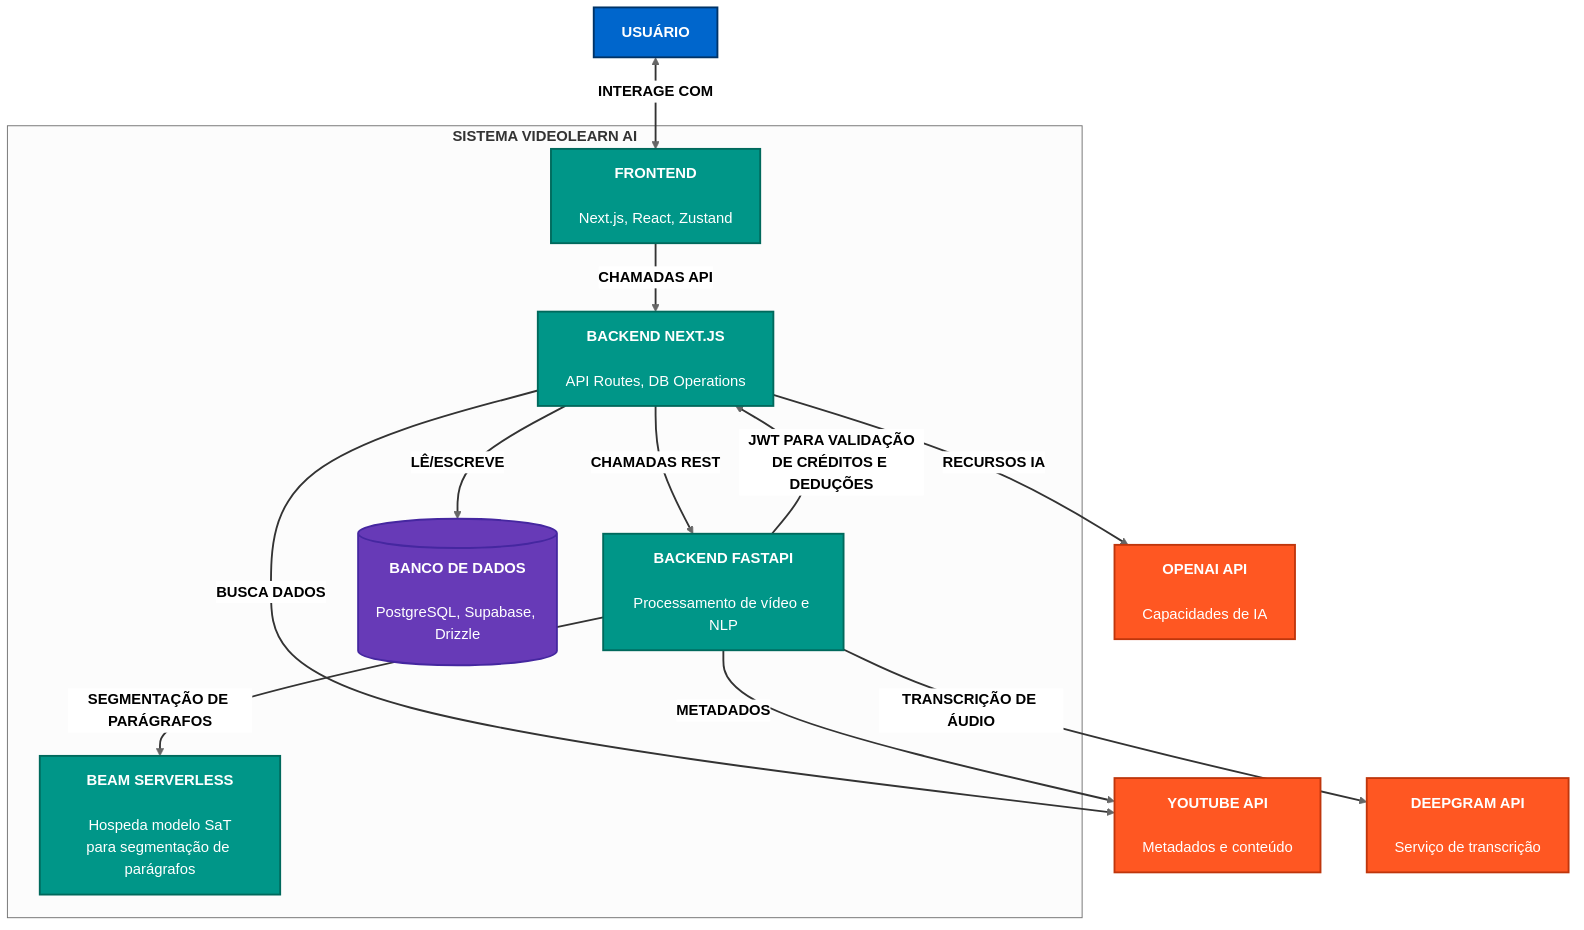
\includegraphics[width=0.95\textwidth,height=0.9\textheight,keepaspectratio]{exemplo-slides/graphics/images/c4_simplified-1.png}
  \caption{Diagrama de arquitetura do sistema VideoLearnAI}
  \label{fig:architecture}
\end{figure}

\subsection{Componentes Principais}

\subsubsection{Frontend}
O frontend da aplicação é construído com Next.js, React e utiliza Zustand para gerenciamento de estado. Esta camada é responsável pela interface do usuário, permitindo interações intuitivas com o conteúdo de vídeo e os recursos de aprendizado. 

\subsubsection{Backend Next.js}
O backend implementado com Next.js API Routes gerencia as operações de banco de dados e integrações com serviços externos. Este componente é o único com acesso direto ao banco de dados, centralizando a lógica de persistência e garantindo a integridade dos dados. Além disso, ele se comunica com APIs externas como YouTube e OpenAI para obter metadados de vídeos e recursos de IA, respectivamente.

\subsubsection{Backend FastAPI}
Desenvolvido em Python, essa camada é especializada em processamento e análise de conteúdo de vídeos do YouTube. Ele extrai metadados, baixa áudio, realiza transcrição automática via Deepgram API e segmenta o texto em parágrafos utilizando o serviço Beam. O sistema implementa autenticação JWT para validar usuários e gerencia créditos através de comunicação com o frontend, deduzindo-os conforme o tempo de vídeo processado.
A arquitetura é modular, com rotas específicas para cada funcionalidade: obtenção de dados do vídeo, download de áudio, transcrição, segmentação de texto e pesquisa. O backend não acessa diretamente o banco de dados, mas se comunica com o frontend para validação de usuários e gerenciamento de créditos, garantindo controle de acesso e uso dos recursos.

\subsubsection{Beam Serverless}
Esta camada hospeda o modelo SaT (Segment Any Text), especializado na segmentação de parágrafos. O Beam Serverless permite a execução eficiente de modelos de IA sem a necessidade de gerenciar infraestrutura, oferecendo escalabilidade automática conforme a demanda e pagando apenas pelo tempo de execução.

\subsubsection{Banco de Dados}
O sistema utiliza PostgreSQL como banco de dados relacional, gerenciado através do Supabase e com esquema definido pelo Drizzle ORM. Esta combinação oferece robustez para armazenamento de dados estruturados, incluindo informações de usuários, conteúdo de vídeos, transcrições e outros dados essenciais para o funcionamento da plataforma.

\subsection{Integrações Externas}

\begin{itemize}
    \item \textbf{YouTube API}: Fornece metadados e conteúdo de vídeos, permitindo que a plataforma acesse informações como título, descrição, duração e outros detalhes relevantes dos vídeos.
    
    \item \textbf{OpenAI API}: Oferece capacidades avançadas de IA para processamento de texto, sendo utilizada pelo backend Next.js para gerar conteúdo enriquecido, como resumos, perguntas e respostas, e outros recursos educacionais baseados no conteúdo dos vídeos.
    
    \item \textbf{Deepgram API}: Serviço especializado em transcrição de áudio, utilizado pelo backend FastAPI para converter o áudio dos vídeos em texto, possibilitando a análise e processamento posterior do conteúdo.
\end{itemize}

\subsection{Fluxos de Comunicação}

Os principais fluxos de comunicação entre os componentes incluem:

\begin{enumerate}
    \item \textbf{Interação do Usuário}: Os usuários interagem com o frontend da aplicação, que apresenta a interface e gerencia as interações.
    
    \item \textbf{Processamento de Dados e Validação de Créditos}: O frontend faz chamadas API para o backend Next.js, que por sua vez pode fazer chamadas REST para o backend FastAPI quando necessário processamento especializado. A comunicação bidirecional entre os backends utiliza tokens JWT para autenticação e autorização, garantindo a segurança e integridade das requisições. Este mecanismo também permite que o backend FastAPI valide e deduza créditos dos usuários através do backend Next.js, assegurando que apenas usuários autorizados acessem recursos premium.
    
    \item \textbf{Segmentação de Parágrafos}: O backend FastAPI se comunica com o Beam Serverless para realizar a segmentação de parágrafos utilizando o modelo SaT.
    
    \item \textbf{Transcrição de Áudio}: O backend FastAPI utiliza o Deepgram API para transcrever o áudio dos vídeos em texto.
    
    \item \textbf{Acesso a Dados}: O backend Next.js é responsável por ler e escrever no banco de dados PostgreSQL através do Supabase e Drizzle ORM.
\end{enumerate}

Esta arquitetura modular permite que o sistema seja escalável, manutenível e extensível, facilitando a adição de novos recursos e a otimização de componentes existentes. A separação clara de responsabilidades entre os diferentes backends e a utilização de serviços especializados para tarefas específicas contribuem para a eficiência e robustez do sistema VideoLearnAI.

\section{Melhoria da Legibilidade das Legendas}

Para resolver o desafio de aprimorar a legibilidade das legendas, foram exploradas duas abordagens distintas. Inicialmente, testou-se uma solução baseada em LLMs (Large Language Models) combinada com um sistema de validação do resultado. Posteriormente, realizou-se uma segunda implementação, dessa vez utilizando o modelo SaT (Segment Any Text). Essa última abordagem se mostrou mais promissora.

\subsection{O Problema da Legibilidade}

As legendas de vídeos frequentemente apresentam problemas de formatação e segmentação, dificultando a compreensão do conteúdo. Esse problema ocorre porque as transcrições brutas costumam ser geradas como um fluxo contínuo de palavras, sem uma estrutura clara de frases e parágrafos. Não foram construídas tendo em mente a leitura da transcrição como um todo e sim apenas aparecer na tela no momento certo.

A disponibilização da transcrição com boa legibilidade, lado a lado com com o conteúdo audiovisual traz diversos benefícios para o processo de aprendizagem. Primeiro, permite que o usuário rapidamente navegue pelo conteúdo, identificando e pulando seções menos relevantes para seu objetivo de estudo. Segundo, quando algum trecho do vídeo não foi bem compreendido, a possibilidade de reler a transcrição daquela parte específica oferece uma abordagem alternativa para entender o conteúdo. Por fim, a integração entre vídeo e transcrição oferece navegação bidirecional: além de realçar automaticamente o texto conforme o vídeo progride, permite saltar para qualquer momento do vídeo com um clique na transcrição, tornando a experiência do usuário mais fluida e interativa.

Na aplicação desenvolvida, o foco foi especificamente na melhoria da segmentação do texto em frases e parágrafos. Embora existam modelos promissores para adicionar pontuação adequada ao texto, como em \cite{guhr-EtAl:2021:fullstop} que utiliza transformers multilíngues para essa tarefa obtendo F1-score médio de 0,94 para detecção de final de sentença em textos em inglês, alemão, francês e italiano, essa funcionalidade será explorada em uma iteração futura do projeto.







\subsection{Primeira Abordagem com LLMs}
Inicialmente, foi utilizado um modelo de linguagem de grande porte (LLM) para segmentar e melhorar a legibilidade do texto das legendas. A implementação foi feita utilizando a biblioteca \texttt{instructor}, que permite a validação do texto gerado através dos modelos de tipagem do \texttt{pydantic}, garantindo conformidade com um formato estruturado.


Para evitar alterações indesejadas no conteúdo original, no modelo Pydantic utilizado, adicionou-se o decorador \verb|@field_validator| para executar
uma função de validação customizada. Esta função utilizava a normalização
de texto para checar se apenas espaços e pontuações foram modificados
entre o texto processado e o original. 

Quando a validação falhava, a
biblioteca instructor automaticamente incluía no proximo prompt o texto
original, a saída que falhou e o erro específico da validação, facilitando que a LLM corrigisse seus erros. Este processo
se repetia automaticamente por até 5 tentativas (definido por
\verb|max_retries=5|) para cada texto processado.

Entretanto, essa abordagem apresentou desafios significativos:
\begin{itemize}
  \item \textbf{Latência elevada}: O processo todo acaba sendo muito demorado pois necessita de várias interações devido a limitação da janela de contexto. Tornando a solução pouco eficiente para processar legendas de vídeos de longa duração
  \item \textbf{Custo financeiro elevado}: O uso de LLMs para processamento de texto em larga escala mostrou-se financeiramente custoso, considerando o volume de requisições necessárias.
  \item \textbf{Alterações não desejadas no texto}: Apesar das instruções explícitas no prompt para evitar adições ou remoções de palavras, o modelo ocasionalmente incluía frases como "Aqui está o seu texto com legibilidade aprimorada" ou alterava partes do conteúdo original, omissão de algumas palavras ou frases por exemplo.
  \item \textbf{Falhas no processo}: Mesmo com o mecanismo de validação e o sistema de retentativas implementados, havia casos em que o processo esgotava o número máximo de iterações sem terminar sem erros.
\end{itemize}

Esses fatores tornaram a abordagem com LLMs inviável para o problema proposto.

\subsection{Implementação com SaT (Segment Anything Text)}

Diante das limitações arquiteturais dos LLMs, discutidas na seção 3.1.5 sobre limitações fundamentais dos modelos de linguagem, foi adotado o SAT (\textit{Segment Any Text}) \cite{frohmann2024segment}, um transformer especializado para segmentação de texto que oferece uma solução mais robusta e eficiente para a melhoria da legibilidade das legendas. Diferente dos LLMs que focam em geração de texto, o SAT utiliza uma arquitetura de classificação binária que apenas identifica os limites entre sentenças, apresentando as seguintes vantagens:

\begin{itemize}
    \item \textbf{Baixa latência:} A segmentação ocorre de maneira rápida e eficiente graças à sua arquitetura otimizada com tokenização por subpalavras com apenas 3 camadas transformer, resultando em um modelo muito menor e especializado para a tarefa.
    
    \item \textbf{Preservação do conteúdo original:} O modelo não gera ou modifica texto, apenas classifica as posições como limites de sentença ou não. Esta abordagem focada em classificação binária garante tanto a fidelidade ao texto original quanto maior confiabilidade e previsibilidade no processamento das legendas.
    
    \item \textbf{Escalabilidade:} Por ser um modelo mais leve, o SAT pode processar textos longos com menor consumo de recursos computacionais, tornando-o ideal para aplicações em produção com restrições de custo e latência.
    
    \item \textbf{Precisão:} Apesar de sua simplicidade relativa, o modelo demonstrou alta precisão na identificação de limites de parágrafos, resultando em textos bem estruturados e de fácil leitura.
\end{itemize}

A implementação do SAT no VideoLearnAI foi realizada através de um serviço dedicado no backend Python (FastAPI), que se comunica com a infraestrutura Beam Serverless GPU para processamento eficiente. O fluxo operacional envolve o recebimento da legenda bruta pelo FastAPI, remoção das informações de tempo (timestamps) para preparar o texto puro, envio ao Beam Serverless para execução do modelo SAT, identificação dos limites de parágrafos, retorno ao FastAPI para reintegração das informações temporais originais ao texto já segmentado, e finalmente formatação do texto estruturado para apresentação ao usuário. Esta arquitetura preserva a sincronização precisa entre o texto segmentado e o vídeo, permitindo que o usuário navegue pelo conteúdo audiovisual através da transcrição, resultando em uma melhoria significativa na legibilidade sem perder a funcionalidade de navegação temporal.

\subsection{Interface e Experiência do Usuário}

\begin{figure}[H]
  \centering
  \begin{subfigure}{0.48\textwidth}
    
\includegraphics[width=\textwidth,height=0.3\textheight,keepaspectratio]{exemplo-slides/graphics/images/dropdown.png}
    \caption{Dropdown de seleção de modo de exibição de legendas}
    \label{fig:dropdown_closed}
  \end{subfigure}
  \hfill
  \begin{subfigure}{0.48\textwidth}
    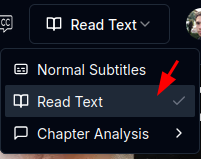
\includegraphics[width=\textwidth,height=0.3\textheight,keepaspectratio]{exemplo-slides/graphics/images/dropdown-aberto.png}
    \caption{Dropdown aberto mostrando as opções disponíveis}
    \label{fig:dropdown_open}
  \end{subfigure}
  \caption{Interface para seleção do modo de leitura da transcrição}
  \label{fig:dropdown_interface}
\end{figure}

Para melhorar a legibilidade do texto das legendas, o usuário pode utilizar o dropdown de seleção mostrado na Figura \ref{fig:dropdown_interface}. Ao clicar neste elemento de interface (Figura \ref{fig:dropdown_closed}), são apresentadas duas opções: "Normal Subtitle" e "Read Text" (Figura \ref{fig:dropdown_open}). Ao selecionar a opção "Read Text", o sistema inicia o processamento para melhorar a legibilidade das legendas, exibindo um toast informativo que indica que o processo está em andamento.

O sistema foi projetado para otimizar a experiência do usuário através do armazenamento de resultados prévios. Quando um vídeo já teve suas legendas processadas anteriormente, o resultado é recuperado automaticamente do banco de dados e o dropdown é inicializado com a opção "Read Text" selecionada. Caso contrário, a opção padrão "Normal Subtitle" é apresentada, permitindo que o usuário solicite o processamento quando desejar.

\begin{figure}[H]
  \centering
  \begin{subfigure}{0.49\textwidth}
    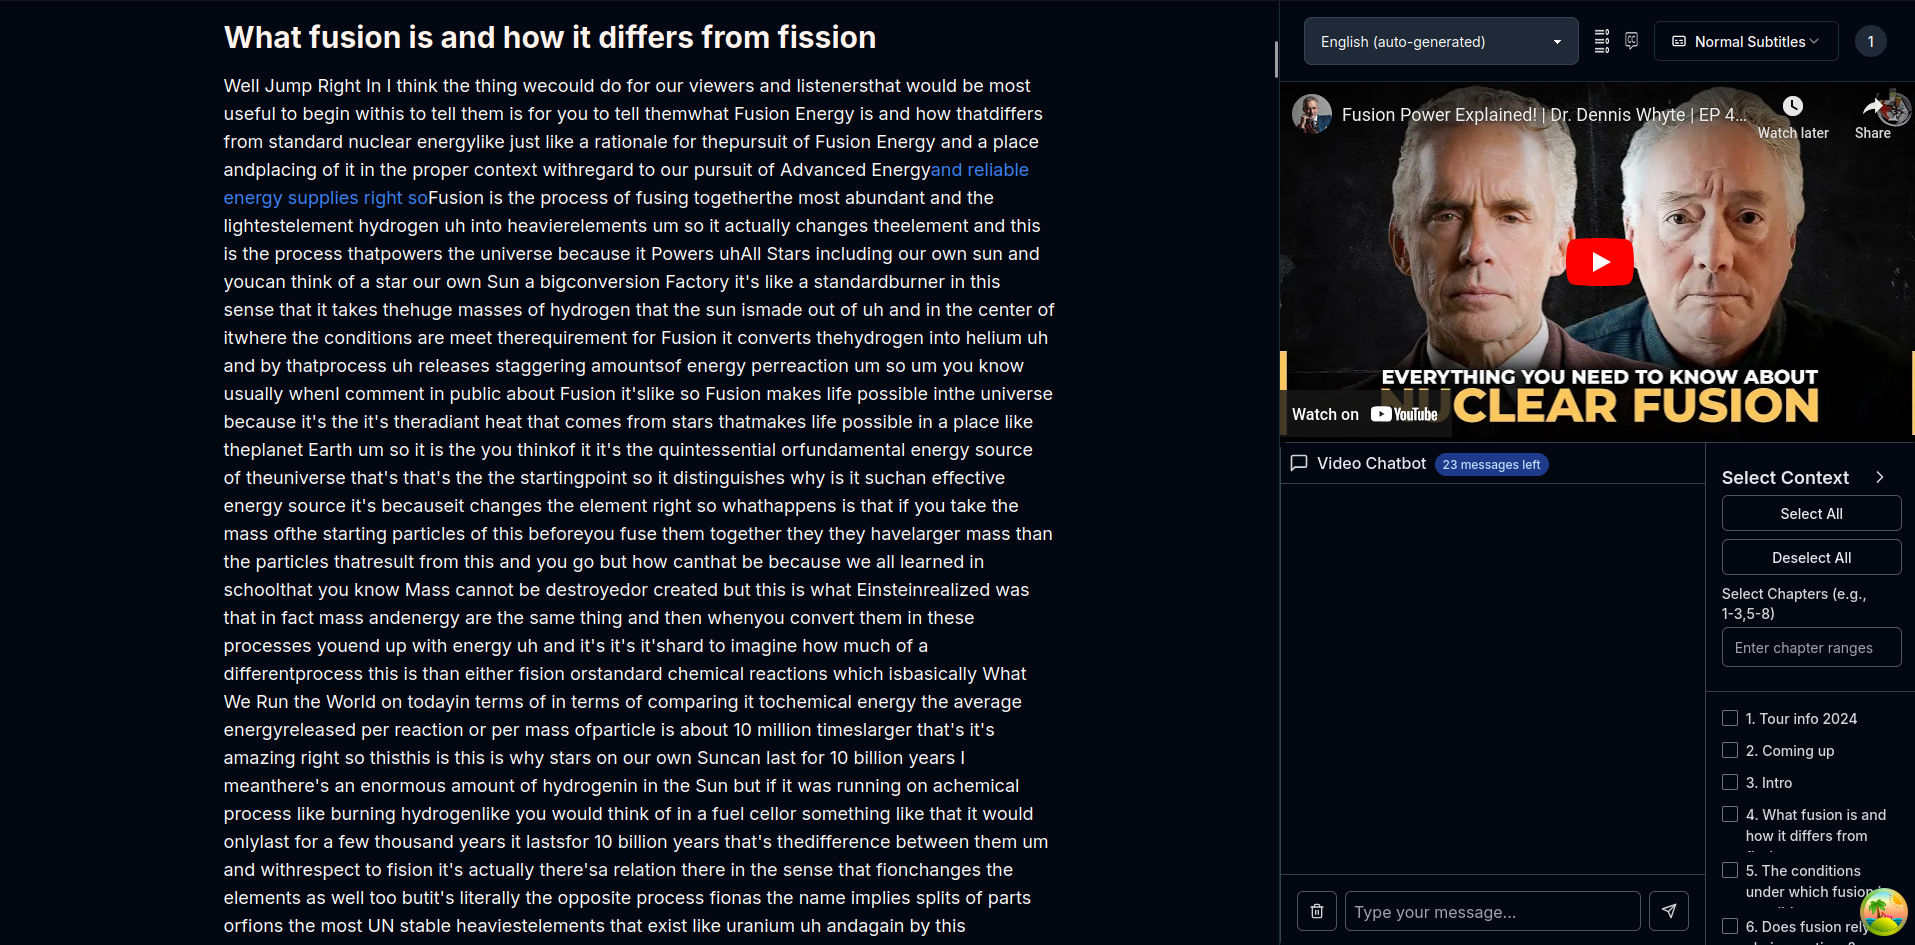
\includegraphics[width=\textwidth,height=0.35\textheight,keepaspectratio]{exemplo-slides/graphics/images/pre-improved-readability.png}
    \caption{Legendas originais sem processamento}
    \label{fig:before_readability}
  \end{subfigure}
  \hfill
  \begin{subfigure}{0.49\textwidth}
    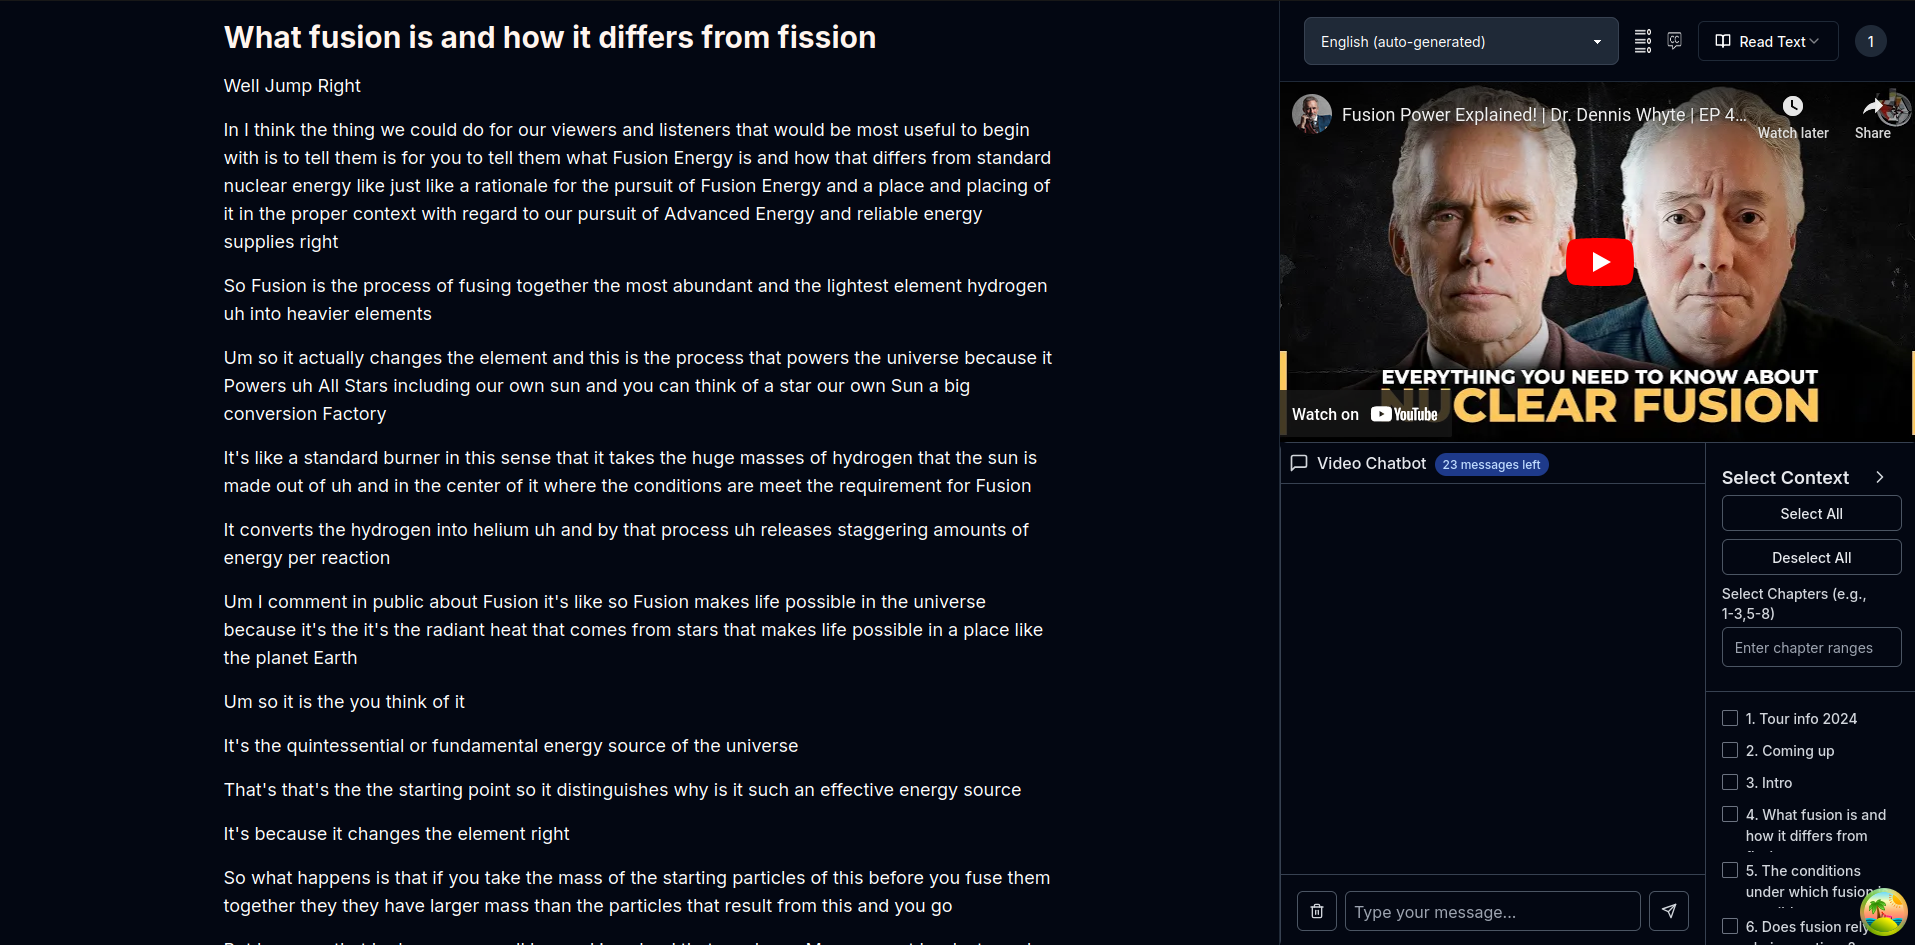
\includegraphics[width=\textwidth,height=0.35\textheight,keepaspectratio]{exemplo-slides/graphics/images/after-improved-readability.png}
    \caption{Legendas após processamento com SAT}
    \label{fig:after_readability}
  \end{subfigure}
  \caption{Comparação da legibilidade antes e depois do processamento com o modelo SAT}
  \label{fig:readability_comparison}
\end{figure}

A Figura \ref{fig:readability_comparison} demonstra o impacto visual da melhoria de legibilidade proporcionada pelo modelo SAT. À esquerda (Figura \ref{fig:before_readability}), observa-se a transcrição original com texto contínuo e sem estruturação clara, dificultando a leitura e compreensão. À direita (Figura \ref{fig:after_readability}), o mesmo conteúdo após o processamento apresenta uma organização em parágrafos lógicos, com espaçamento adequado e estrutura visual que facilita o acompanhamento do conteúdo.

O processamento é realizado de forma eficiente pela infraestrutura Beam Serverless GPU, como evidenciado pelos logs de execução na Figura \ref{fig:beam_logs_cold_start}. Nota-se que, embora exista um tempo inicial de carregamento (cold start) de aproximadamente 18 segundos na primeira requisição, as requisições subsequentes são processadas em apenas 50-100ms. Esta otimização de performance é crucial para a experiência do usuário, garantindo que, após o carregamento inicial, a interação com o sistema seja fluida e responsiva, mesmo ao processar vídeos de longa duração.

\begin{figure}[H]
  \centering
  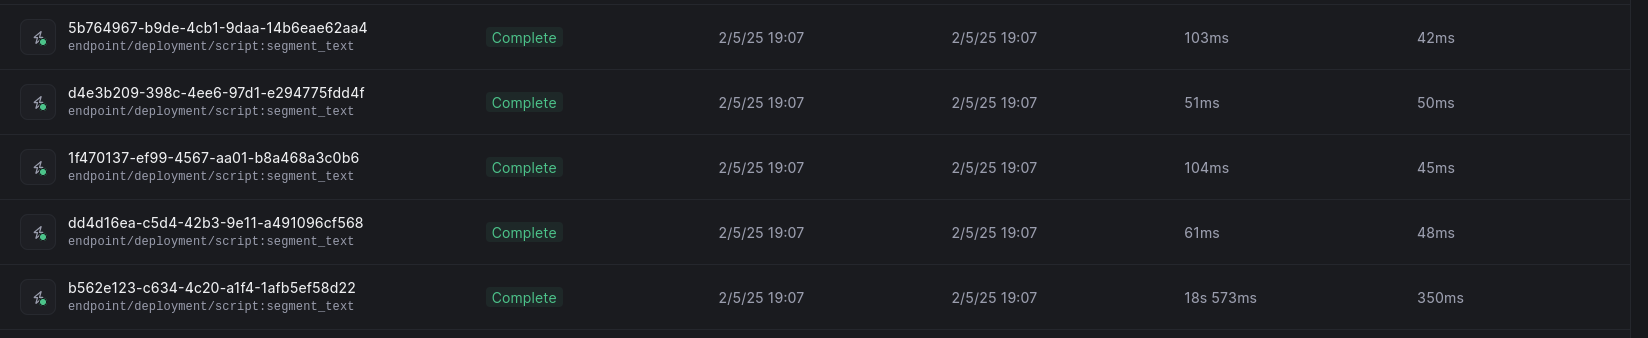
\includegraphics[width=\textwidth,height=0.45\textheight,keepaspectratio]{exemplo-slides/graphics/images/logs-beam.png}
  \caption{Logs de execução no Beam Serverless GPU demonstrando o tempo de cold start (18s 573ms) na primeira requisição e tempos de resposta reduzidos (aproximadamente 50-100ms) nas requisições subsequentes}
  \label{fig:beam_logs_cold_start}
\end{figure}

\section{Gera\c{c}\~{a}o de Cap\'{i}tulos}

A geração automática de capítulos para vídeos do YouTube facilita a navegação e compreensão do conteúdo, organizando transcrições longas em seções temáticas. Esta funcionalidade permite que os usuários localizem rapidamente informações específicas e compreendam melhor a estrutura do material apresentado.

\subsection{Arquitetura do Sistema de Geração de Capítulos}

O sistema implementado no VideoLearnAI utiliza uma abordagem em duas etapas que combina segmentação de texto e processamento de linguagem natural para identificar transições temáticas em transcrições de vídeo:

\begin{enumerate}
    \item \textbf{Segmentação de Parágrafos com o Modelo SAT}: Inicialmente, a transcrição completa do vídeo é processada pelo modelo SAT (Segment Any Text), que identifica fronteiras naturais de parágrafos baseando-se no contexto semântico.

    \item \textbf{Identificação de Transições Temáticas via LLM}: Os parágrafos segmentados são então analisados por um modelo de linguagem grande (LLM) que identifica mudanças significativas de tópico e gera títulos descritivos para cada seção.
\end{enumerate}

Esta abordagem híbrida aproveita as forças complementares de cada modelo: a precisão do SAT na segmentação estrutural do texto e a capacidade do LLM de compreender contexto semântico e identificar transições temáticas.

\subsection{Fluxo de Processamento}

O processo de geração de capítulos segue um fluxo bem definido:

\begin{enumerate}
    \item \textbf{Estruturação do texto}: A transcrição do vídeo é segmentada em parágrafos coerentes utilizando o modelo SAT, que compreende o contexto semântico e identifica fronteiras naturais no texto, mesmo em transcrições que carecem de pontuação adequada.

    \item \textbf{Numeração dos parágrafos}: Cada parágrafo recebe um identificador numérico sequencial e é associado ao seu timestamp de início correspondente. Esta associação é fundamental para o mapeamento posterior entre os capítulos identificados e os momentos específicos do vídeo.

    \item \textbf{Identificação de transições temáticas}: O texto segmentado e numerado é enviado para um LLM (especificamente o GPT-4o) através de uma prompt cuidadosamente elaborada. A prompt instrui o modelo a identificar onde novos capítulos devem começar e a gerar títulos descritivos para cada seção.

    \item \textbf{Transformação em capítulos sincronizados}: Os tópicos identificados pelo LLM são transformados em capítulos sincronizados com o vídeo, mapeando os números de parágrafo para os timestamps correspondentes. Cada capítulo contém um título, tempos de início e término, e um estado de ativação para indicar se o capítulo está ativo ou não na interface.
\end{enumerate}

\subsection{Integração com LLMs via Function Calling}

Para a identificação das transições de tópico, o sistema utiliza function calling para interagir com o LLM. Esta abordagem estruturada permite enviar a transcrição segmentada e numerada, solicitando ao modelo que retorne uma lista de objetos representando os pontos de mudança mais relevantes.

\begin{figure}[H]
  \centering
  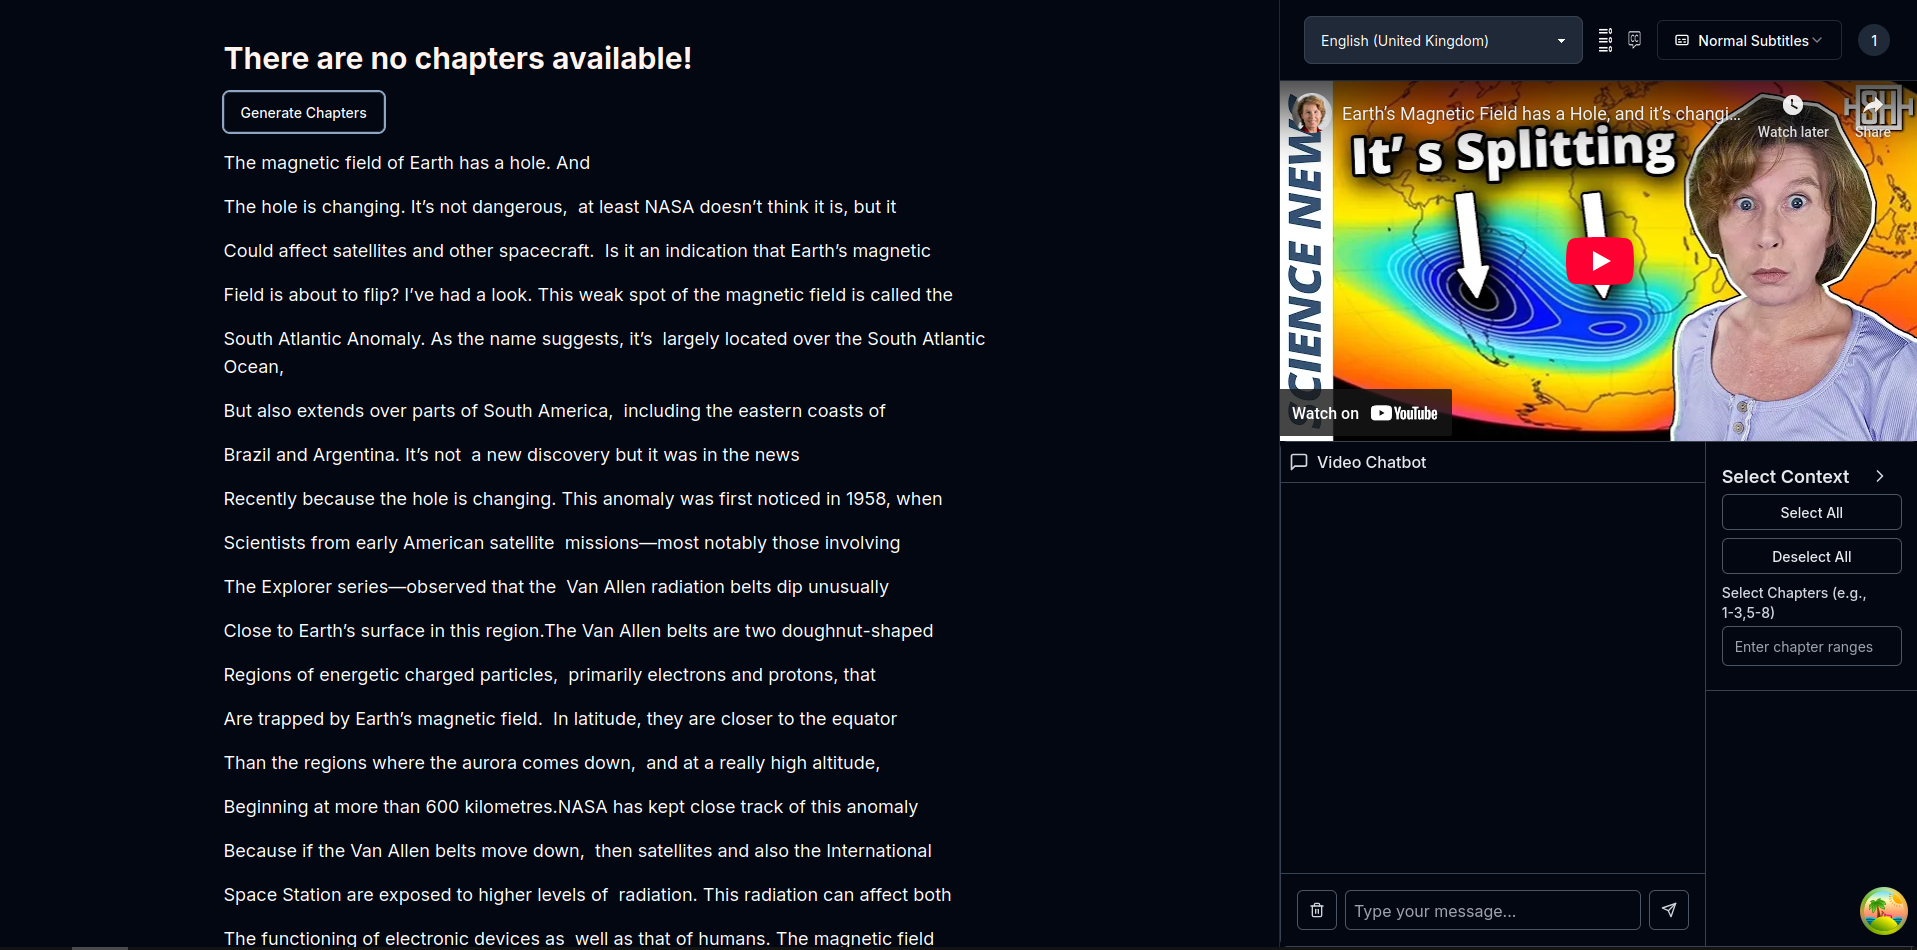
\includegraphics[width=\textwidth,height=0.45\textheight,keepaspectratio]{exemplo-slides/graphics/images/generate-chapters.png}
  \caption{Interface para iniciar o processo de geração automática de capítulos, mostrando o botão "Generate Chapters" que aciona o processamento}
  \label{fig:generate_chapters}
\end{figure}

Como mostrado na Figura \ref{fig:generate_chapters}, o usuário pode iniciar o processo de geração de capítulos através de um botão dedicado na interface. Ao clicar neste botão, o sistema inicia o processamento da transcrição, aplicando primeiro a segmentação de parágrafos e em seguida a análise semântica para identificação de tópicos.

A função chamada retorna uma lista estruturada de tópicos, cada um contendo um título descritivo e o número do parágrafo onde o capítulo começa. Esta abordagem estruturada facilita o processamento posterior e a sincronização com o vídeo.

Inicialmente, foi testada uma abordagem em que o LLM era solicitado a identificar diretamente os tópicos e seus timestamps correspondentes. No entanto, esta tarefa mostrou-se excessivamente complexa para o modelo, resultando em frequentes imprecisões temporais. A solução implementada simplifica significativamente o problema: em vez de exigir que o LLM compreenda e gere informações temporais precisas, o sistema solicita apenas a identificação dos números dos parágrafos onde ocorrem transições temáticas.

Esta estratégia reduz a complexidade cognitiva para o LLM, permitindo que ele se concentre exclusivamente na análise semântica do conteúdo - tarefa para a qual é naturalmente otimizado. O mapeamento entre parágrafos e timestamps é realizado posteriormente pelo sistema, utilizando as associações temporais já estabelecidas durante a segmentação inicial. 

\begin{figure}[H]
  \centering
  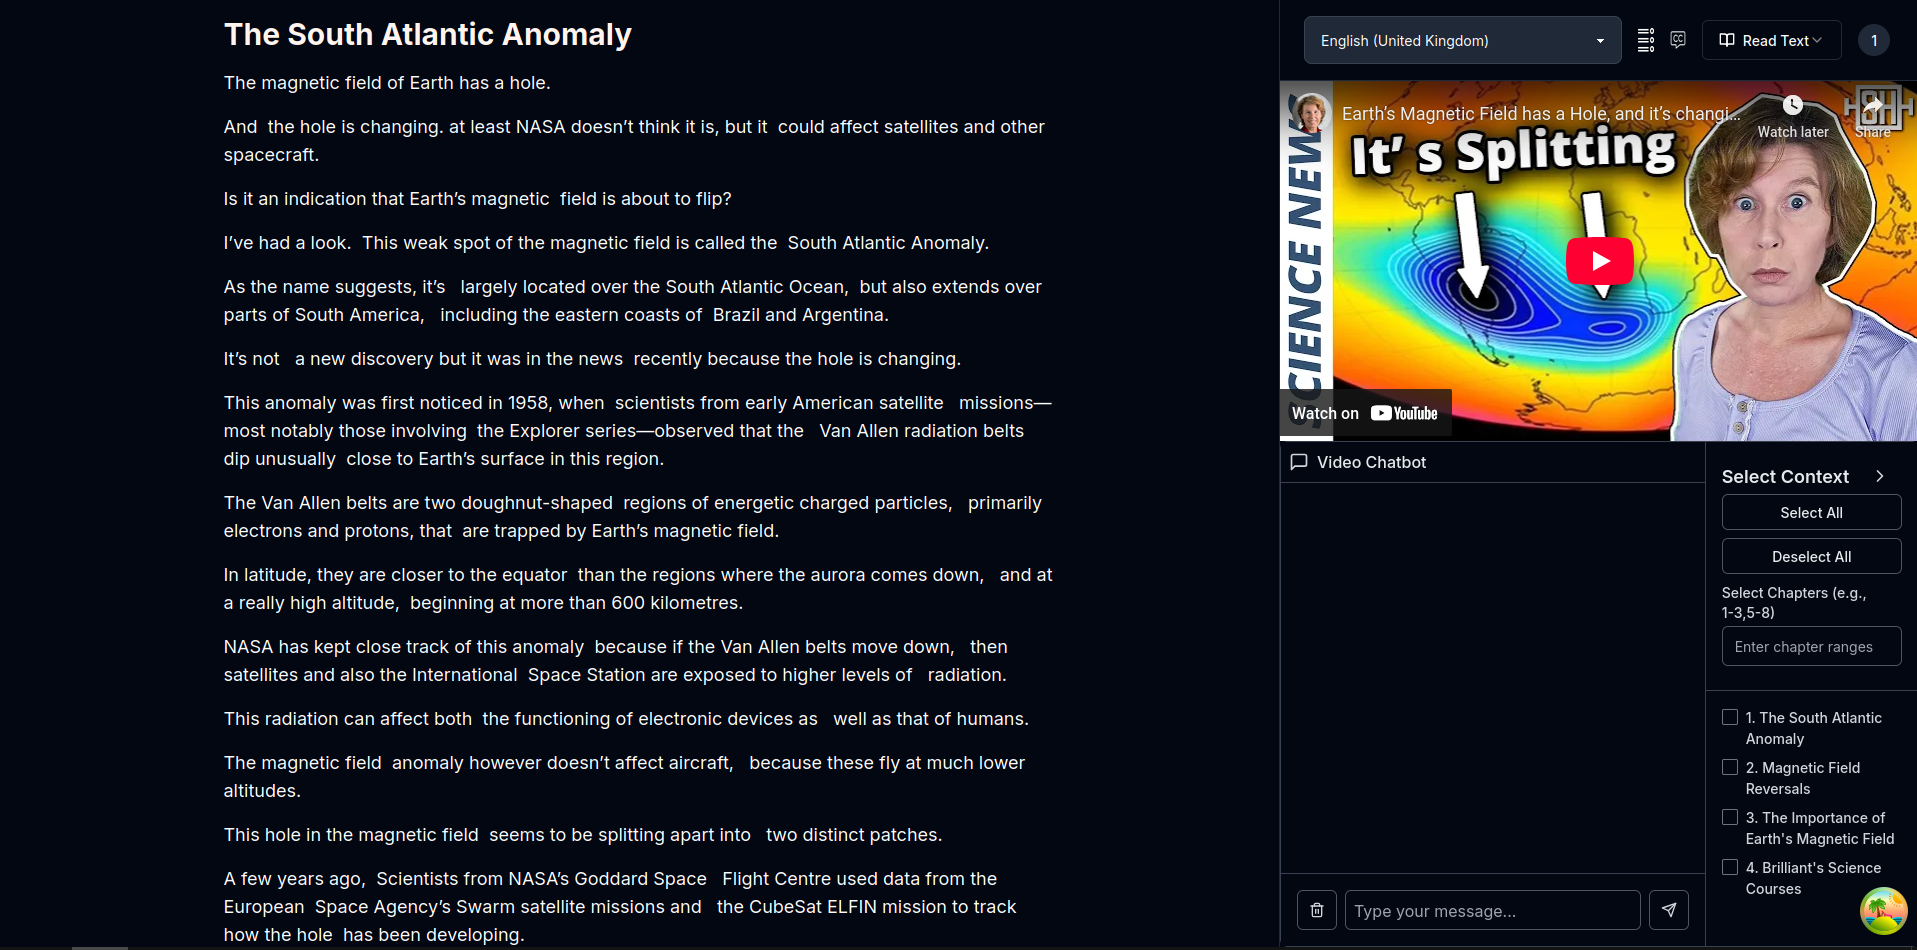
\includegraphics[width=\textwidth,height=0.45\textheight,keepaspectratio]{exemplo-slides/graphics/images/after-chapter-generation.png}
  \caption{Interface após a geração de capítulos, os capítulos são listados no contexto do Chat e também na tabela de conteúdos que será apresentada na próxima seção}
  \label{fig:after_chapter_generation}
\end{figure}

O resultado do processo de geração de capítulos é ilustrado na Figura \ref{fig:after_chapter_generation}, onde se pode observar a interface atualizada com a lista de capítulos gerados. 



\subsection{Tabela de Conteúdos e Histórico de Visualização}

Os capítulos gerados automaticamente servem como fundamento para recursos adicionais que enriquecem a experiência de aprendizagem. Dois desses recursos são particularmente importantes: o Sumário de Conteúdo e o Histórico de Visualização com Progresso.

\begin{figure}[H]
  \centering
  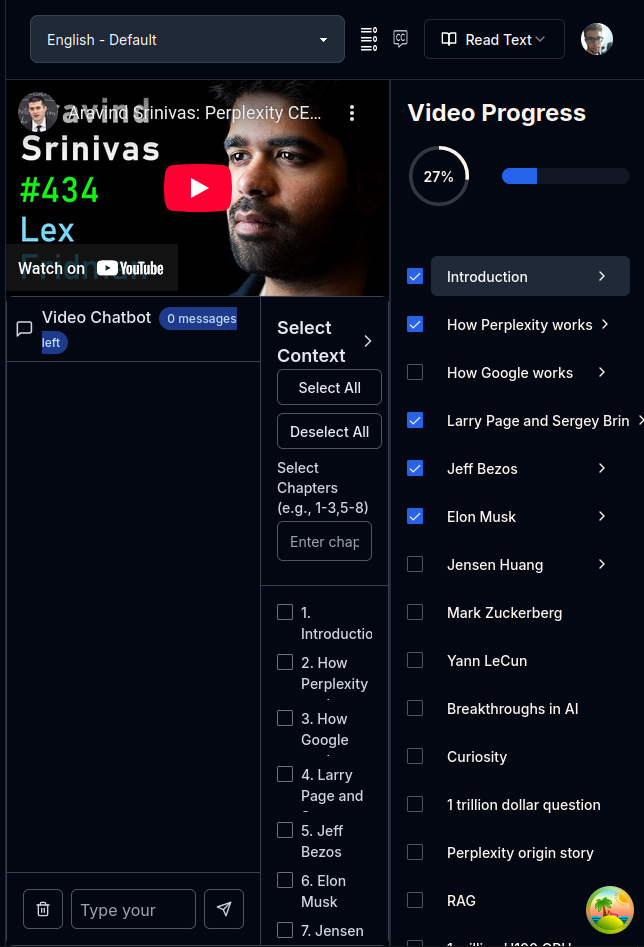
\includegraphics[width=\textwidth,height=0.45\textheight,keepaspectratio]{exemplo-slides/graphics/images/table of contents.png}
  \caption{Interface do Sumário de Conteúdo, mostrando a lista de capítulos com indicadores de progresso e opções para marcar capítulos como concluídos}
  \label{fig:table_of_contents}
\end{figure}

Como ilustrado na Figura \ref{fig:table_of_contents}, o sistema oferece um Sumário de Conteúdo acessível através de um botão localizado ao lado do seletor de transcrição. Este recurso apresenta uma visão estruturada de todos os capítulos do vídeo, permitindo que o usuário:

\begin{itemize}
    \item Navegue diretamente para qualquer capítulo com um clique, alterando automaticamente a posição do vídeo e o scroll da transcrição
    \item Marque capítulos individuais como concluídos, facilitando o acompanhamento do progresso de estudo
    \item Visualize o percentual total de conclusão do vídeo, baseado nos capítulos marcados como concluídos
\end{itemize}

Esta funcionalidade é particularmente útil para vídeos longos, permitindo que o usuário acompanhe seu progresso e retome o estudo de forma organizada. Vale ressaltar que o sistema funciona tanto com capítulos nativos do YouTube quanto com capítulos gerados automaticamente pela plataforma, garantindo sua utilidade para qualquer tipo de conteúdo.

\begin{figure}[H]
  \centering
  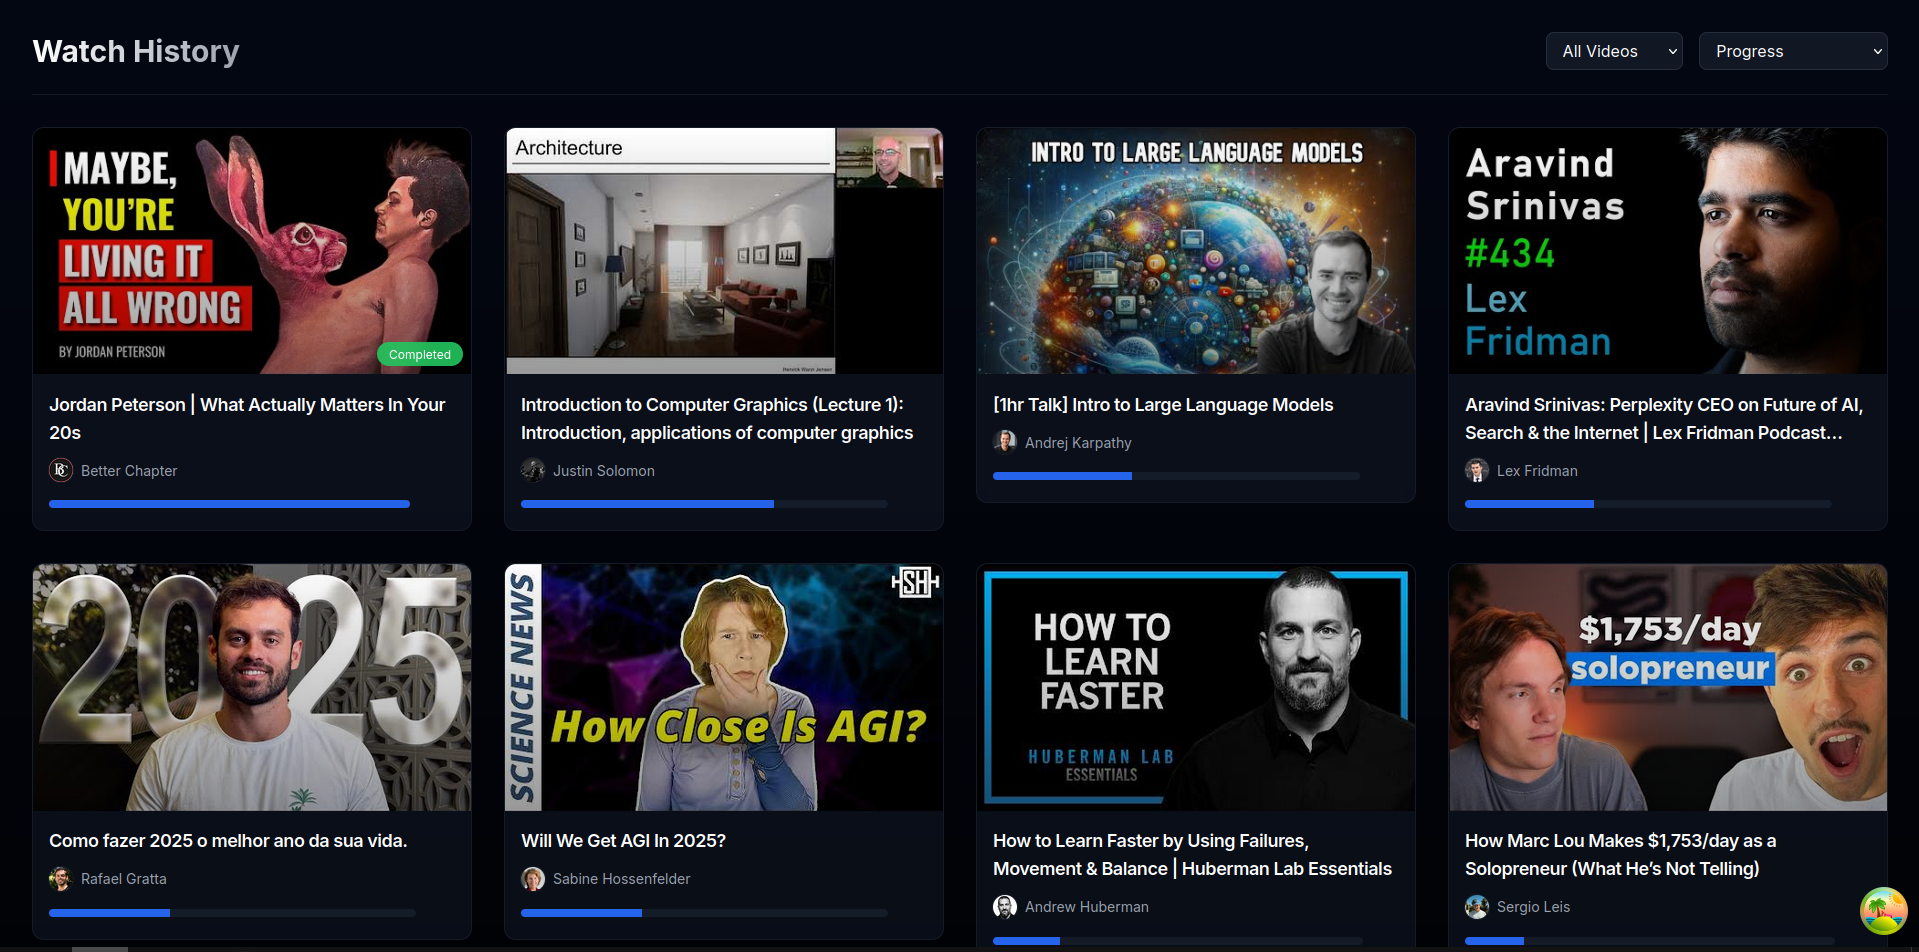
\includegraphics[width=\textwidth,height=0.45\textheight,keepaspectratio]{exemplo-slides/graphics/images/watch history.png}
  \caption{Tela de Histórico de Visualização, exibindo os vídeos assistidos pelo usuário com seus respectivos percentuais de progresso}
  \label{fig:watch_history}
\end{figure}

Complementando o Sumário de Conteúdo, o sistema também oferece uma visão consolidada do progresso através da tela de Histórico de Visualização, mostrada na Figura \ref{fig:watch_history}. Esta interface apresenta todos os vídeos que o usuário começou a assistir, junto com:

\begin{itemize}
    \item O percentual de progresso para cada vídeo, calculado com base nos capítulos marcados como concluídos
    \item Informações básicas sobre cada vídeo, como título e miniatura
    \item Acesso direto para retomar a visualização de qualquer vídeo
\end{itemize}

Este recurso facilita o gerenciamento de múltiplos vídeos de estudo, eliminando a necessidade de lembrar manualmente onde o usuário parou em cada conteúdo e proporcionando uma visão clara de seu progresso geral.

A implementação destas funcionalidades demonstra como a estruturação do conteúdo em capítulos, sejam eles nativos ou gerados automaticamente, pode melhorar significativamente a experiência de aprendizagem com vídeos.

\section{Geração de Transcrição}

A transcrição precisa de vídeos do YouTube é essencial para gerar textos mais confiáveis do que as legendas automáticas, que apresentam qualidade inferior especialmente para línguas que não são o inglês.

\subsection{Primeira implementação com Whisper}

No fluxo original utilizando o Whisper, o processo consistia em:

\begin{enumerate}
    \item \textbf{Download do áudio} (comum a ambos os métodos):
    \begin{itemize}
        \item Uso da biblioteca \texttt{pytubefix} para download
        \item Progresso reportado ao usuário via SSE (Server-Sent Events)
        \item Arquivo de áudio com qualidade balanceada entre precisão e velocidade
    \end{itemize}

    \item \textbf{Pré-processamento específico para Whisper}:
    \begin{itemize}
        \item Divisão do áudio em segmentos de 10 minutos
        \item Cortes preferencialmente em momentos de silêncio
        \item Envio paralelo dos segmentos para transcrição
        \item Necessidade decorrente das limitações do Whisper com arquivos longos
    \end{itemize}
\end{enumerate}

\subsection{Migração para o Deepgram}

Com a adoção do Deepgram, o fluxo foi otimizado:

\begin{enumerate}
    \item \textbf{Download do áudio mantido}:
    \begin{itemize}
        \item Mesmo processo via \texttt{pytubefix} com feedback via SSE
        \item Eliminação da etapa de divisão do áudio
    \end{itemize}

    \item \textbf{Transcrição direta}:
    \begin{itemize}
        \item Envio do arquivo de áudio completo
        \item Processamento único sem necessidade de paralelização
        \item Interface exibe estimativa de tempo restante
        \item Capacidade nativa de lidar com longas durações
    \end{itemize}
\end{enumerate}

\subsection{Interface e Experiência do Usuário}

O processo de transcrição começa quando o usuário clica no botão "CC" localizado na interface principal, como mostrado na Figura \ref{fig:cc_button}.

\begin{figure}[H]
  \centering
  
\includegraphics[width=\textwidth,height=0.45\textheight,keepaspectratio]{exemplo-slides/graphics/images/CC.png}
  \caption{Botão "CC" para iniciar o processo de transcrição}
  \label{fig:cc_button}
\end{figure}

Ao clicar neste botão, é exibido um modal de confirmação que apresenta informações importantes para o usuário: a quantidade de créditos disponíveis em sua conta e a duração do vídeo a ser processado, como ilustrado na Figura \ref{fig:Transcription Modal}.

\begin{figure}[H]
  \centering
  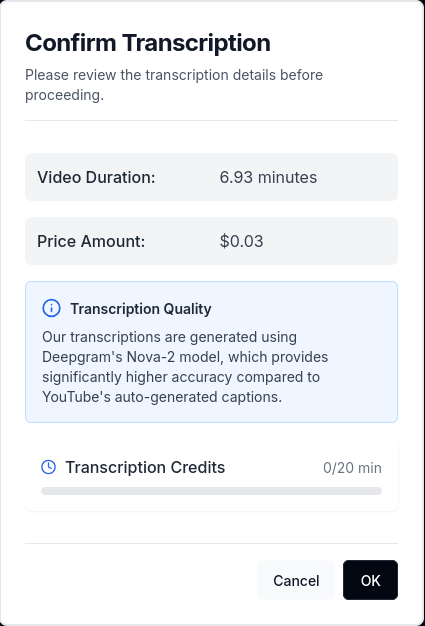
\includegraphics[width=\textwidth,height=0.45\textheight,keepaspectratio]{exemplo-slides/graphics/images/transcription-modal.png}
  \caption{Modal de confirmação mostrando créditos disponíveis e duração do vídeo}
  \label{fig:Transcription Modal}
\end{figure}

Após o usuário confirmar a operação clicando em "OK", o sistema inicia uma série de etapas de processamento. Primeiramente, ocorre a validação da duração do vídeo, onde o backend Next.js verifica a duração real através da API do YouTube. Esta verificação de segurança garante que a informação de duração não tenha sido adulterada no frontend, como mostrado na Figura \ref{fig:validating}.

\begin{figure}[H]
  \centering
  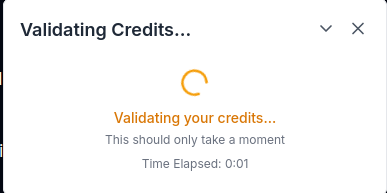
\includegraphics[width=\textwidth,height=0.45\textheight,keepaspectratio]{exemplo-slides/graphics/images/validating.png}
  \caption{Etapa de validação da duração do vídeo via API do YouTube}
  \label{fig:validating}
\end{figure}

Em seguida, o sistema inicia o download do áudio do vídeo. Durante esta etapa, o progresso é exibido em tempo real com atualizações percentuais, permitindo que o usuário acompanhe o andamento do processo, como ilustrado na Figura \ref{fig:downloading}.

\begin{figure}[H]
  \centering
  
\includegraphics[width=\textwidth,height=0.45\textheight,keepaspectratio]{exemplo-slides/graphics/images/downloading.png}
  \caption{Progresso do download do áudio do vídeo com atualização percentual}
  \label{fig:downloading}
\end{figure}

Após o download completo do áudio, inicia-se o processo de transcrição propriamente dito. Diferentemente da etapa de download, a API do Deepgram não fornece atualizações percentuais do progresso. No entanto, o sistema apresenta uma estimativa de tempo restante baseada na velocidade de processamento informada pelo modelo Nova-2 do Deepgram, como mostrado na Figura \ref{fig:transcribing}.

\begin{figure}[H]
  \centering
  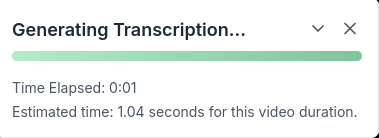
\includegraphics[width=\textwidth,height=0.45\textheight,keepaspectratio]{exemplo-slides/graphics/images/transcribing.png}
  \caption{Processo de transcrição em andamento com estimativa de tempo restante}
  \label{fig:transcribing}
\end{figure}

Após a conclusão do processo, o sistema exibe uma tela de confirmação indicando que a transcrição foi finalizada com sucesso, como ilustrado na Figura \ref{fig:completed-transcription}.

\begin{figure}[H]
  \centering
  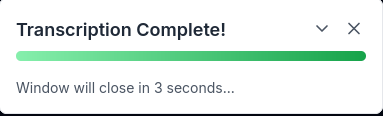
\includegraphics[width=\textwidth,height=0.45\textheight,keepaspectratio]{exemplo-slides/graphics/images/completed-transcription.png}
  \caption{Tela de conclusão do processo de transcrição}
  \label{fig:completed-transcription}
\end{figure}

Após a conclusão bem-sucedida do processo de transcrição, a interface é atualizada automaticamente para exibir o texto transcrito, e o seletor de transcrição adiciona no dropdown o grupo AI transcription e adiciona um item chamado de Transcription. Esse elemento, a transcrição gerada é automaticamente selecionada.
\section{Gera\c{c}\~ao de Quizzes}

A gera\c{c}\~ao de quizzes para cada cap\'{i}tulo representa uma aplica\c{c}\~ao direta dos princ\'{i}pios de aprendizagem ativa discutidos na fundamenta\c{c}\~ao te\'orica. Como visto anteriormente, o ato de testar-se durante o processo de estudo ativa o mecanismo de pr\'atica de recupera\c{c}\~ao, que fortalece significativamente a reten\c{c}\~ao de longo prazo. Esta funcionalidade transforma momentos de consumo passivo em oportunidades de engajamento cognitivo, permitindo que o usu\'ario verifique sua compreens\~ao do conte\'udo antes de avan\c{c}ar para a pr\'oxima se\c{c}\~ao.

Foram desenvolvidas duas interfaces gr\'aficas distintas para os quizzes, adaptadas a diferentes tipos de perguntas:

\begin{itemize}
  \item Interface para questões de \textit{Verdadeiro ou Falso}.
  \item Interface para quest\~oes do tipo \textit{Pergunta e Resposta} (\textit{Q\&A}).
\end{itemize}

Em ambos os casos, a interação com o quiz é implementada de forma dinâmica através do Vercel AI SDK. Esta biblioteca permite que a interface do usuário seja atualizada progressivamente, exibindo as perguntas e respostas à medida que são geradas pela Large Language Model (LLM), sem necessidade de aguardar o processamento completo. Esta abordagem de streaming melhora significativamente a experiência do usuário (UX), reduzindo a percepção de tempo de espera e proporcionando feedback visual imediato durante o processo de geração.

Para garantir a compatibilidade entre as respostas geradas pela LLM e as interfaces gráficas, o sistema utiliza o mecanismo de function calling. Esta técnica, detalhada na fundamentação teórica, permite definir um schema estruturado que a LLM deve seguir ao gerar seu output. Ao especificar o formato exato esperado para as questões e respostas, o sistema consegue processar e renderizar corretamente os elementos de interface em tempo real, eliminando problemas de parsing e garantindo consistência na apresentação dos quizzes.

Além disso, para ambos os tipos de quiz, o usuário tem a opção de personalizar o comportamento da LLM por meio da edição do prompt específico. Esta personalização é acessível através do botão de três pontos na interface do quiz, permitindo ajustes nas diretrizes de geração das questões. O usuário pode, por exemplo, solicitar questões mais desafiadoras, focar em conceitos específicos ou alterar o estilo das perguntas. Esta capacidade de customização torna o sistema adaptável a diferentes objetivos pedagógicos e estilos de aprendizagem, aumentando sua utilidade como ferramenta educacional.

\subsection{Questões discursivas}

\begin{figure}[H]
\centering
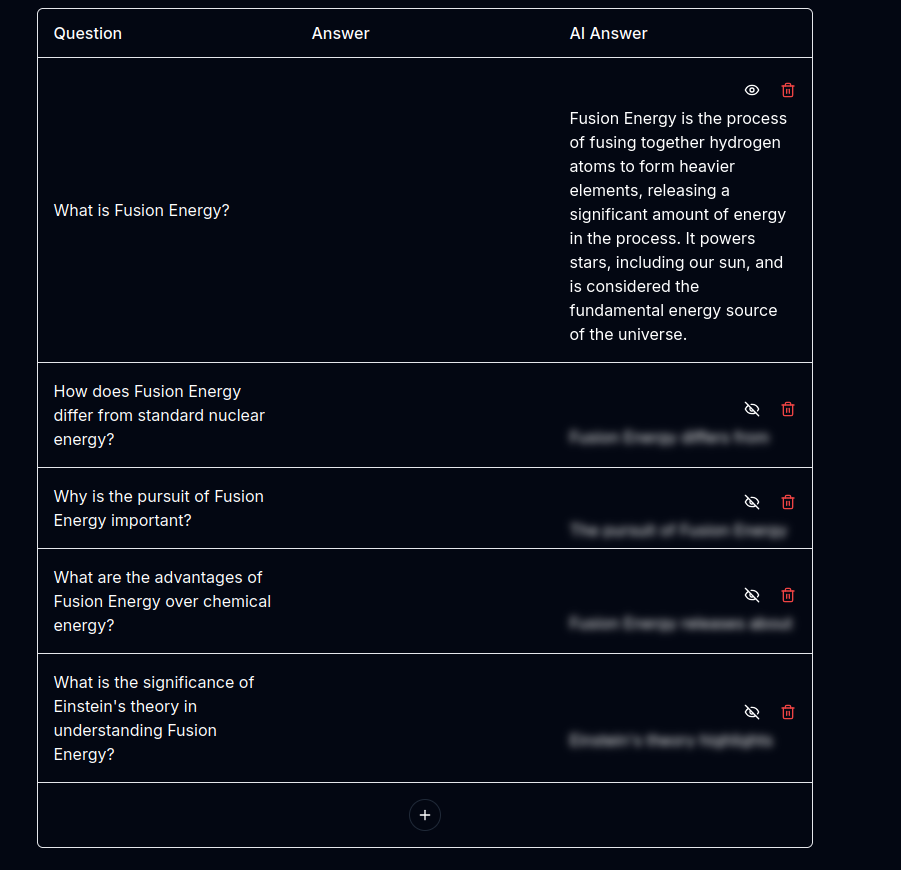
\includegraphics[width=\textwidth,height=0.45\textheight,keepaspectratio]{exemplo-slides/graphics/images/q_a.png}
\caption{Exemplo de interface para perguntas e respostas.}
\label{fig:qa_interface}
\end{figure}

A interface de perguntas e respostas (Q\&A) apresenta uma tabela com três colunas: a primeira exibe a pergunta gerada, a segunda, chamada ``Resposta'', permite ao usuário inserir sua resposta manualmente, e a terceira, ``AI Answer'', que é inicialmente oculta por um efeito de \textit{blur}. A visibilidade dessa coluna pode ser alternada através de um botão, permitindo que o usuário visualize ou oculte a resposta gerada pela IA. O objetivo desse design é incentivar o usuário a tentar responder antes de consultar a resposta fornecida pela IA, promovendo a aprendizagem ativa.


\subsection{Questões de Verdadeiro ou Falso}

\begin{figure}[H]
\centering
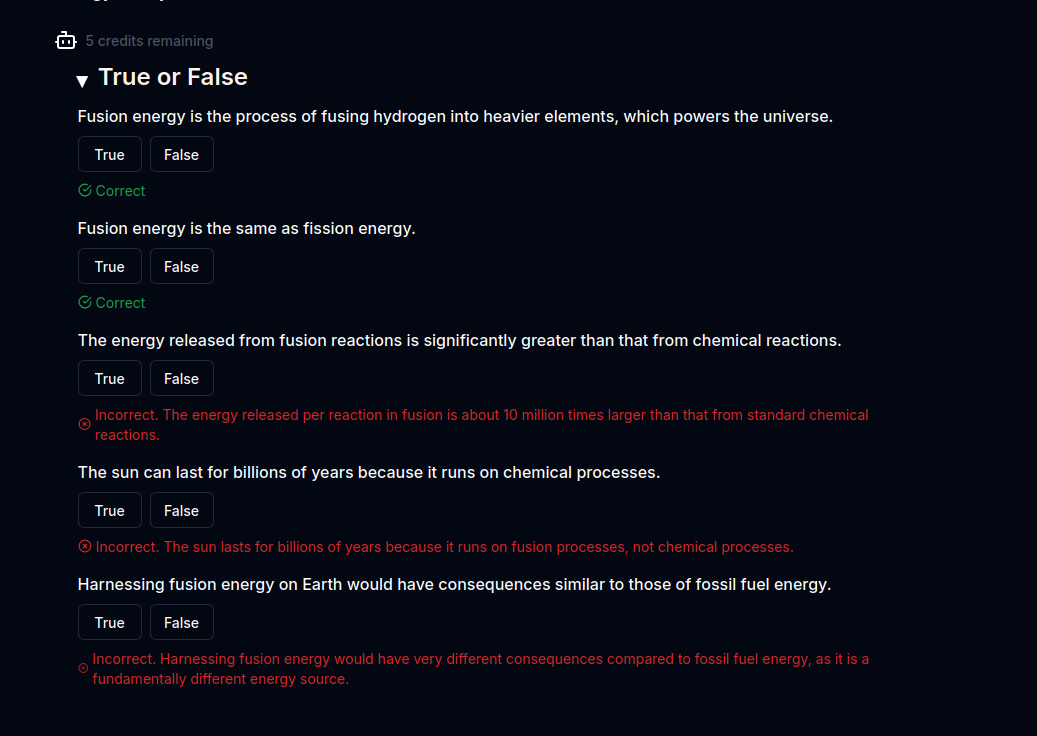
\includegraphics[width=\textwidth,height=0.45\textheight,keepaspectratio]{exemplo-slides/graphics/images/true_or_false.png}
\caption{Exemplo de interface para quest~oes de verdadeiro ou falso.}
\label{fig:true_false_interface}
\end{figure}

Na interface de Verdadeiro ou Falso, as perguntas são apresentadas como afirmações textuais, e abaixo de cada uma há dois botões que permitem ao usuário marcar a resposta como verdadeira ou falsa. Após a seleção um texto adicional surge abaixo, indicando o resultado da resposta: caso esteja correta, a confirmação aparece em verde; caso esteja errada, um texto em vermelho explica o motivo do erro. Esse feedback imediato auxilia na compreensão dos conceitos e melhora a fixação do aprendizado.

\subsection{Geração e Personalização de Quizzes}

Uma característica distintiva do sistema de quizzes implementado é a possibilidade de personalização dos prompts utilizados para gerar as questões. Esta funcionalidade permite que o usuário adapte o comportamento do modelo de linguagem às suas necessidades específicas de aprendizado, seja alterando o estilo, a dificuldade ou mesmo o idioma das questões geradas.

O fluxo de interação para geração e customização de quizzes inicia-se ao final de cada capítulo, onde um botão é apresentado, como ilustrado na Figura \ref{fig:magic_functions}.

\begin{figure}[H]
\centering
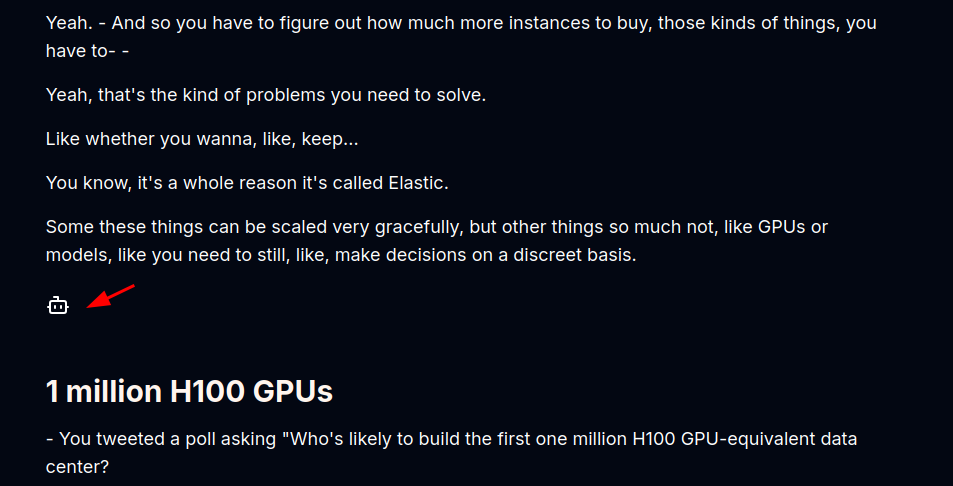
\includegraphics[width=\textwidth,height=0.45\textheight,keepaspectratio]{exemplo-slides/graphics/images/quizzes/botao-magic-functions.png}
\caption{Botão ao final de cada capítulo, oferecendo diferentes opções de interação com o conteúdo}
\label{fig:magic_functions}
\end{figure}

Ao clicar neste botão, o usuário é apresentado a um menu com diferentes opções para interagir com o conteúdo do capítulo. As opções padrão incluem a geração de questões de Verdadeiro ou Falso e perguntas discursivas (Q\&A). Além destas, há uma terceira opção chamada "Custom Text Prompt", que diferentemente das anteriores, não renderiza uma interface específica de quiz, mas processa o texto do capítulo e retorna o resultado como texto simples. Por padrão, esta opção realiza uma sumarização do conteúdo, mas pode ser personalizada para executar qualquer tipo de transformação textual.

Cada uma dessas opções possui dois elementos: um botão principal com o nome da funcionalidade, que ao ser clicado gera imediatamente o resultado usando o prompt padrão, e um botão de três pontos adjacente que oferece possibilidade de customização do prompt, como mostrado na Figura \ref{fig:three_dots}.

\begin{figure}[H]
\centering
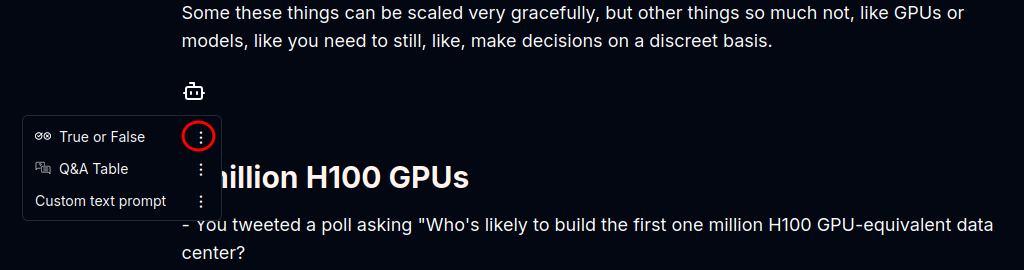
\includegraphics[width=\textwidth,height=0.45\textheight,keepaspectratio]{exemplo-slides/graphics/images/quizzes/three-dots.png}
\caption{Botão de três pontos para acesso a customização do prompt, nesse caso específico para a opção de geração de questões de Verdadeiro ou Falso}
\label{fig:three_dots}
\end{figure}

Ao clicar no botão de três pontos ao lado da opção desejada (Verdadeiro ou Falso, Q\&A ou Custom Text Prompt), um popover é exibido contendo um campo de texto onde o usuário pode inserir instruções personalizadas para o modelo de linguagem, como ilustrado na Figura \ref{fig:custom_prompt}.

\begin{figure}[H]
\centering
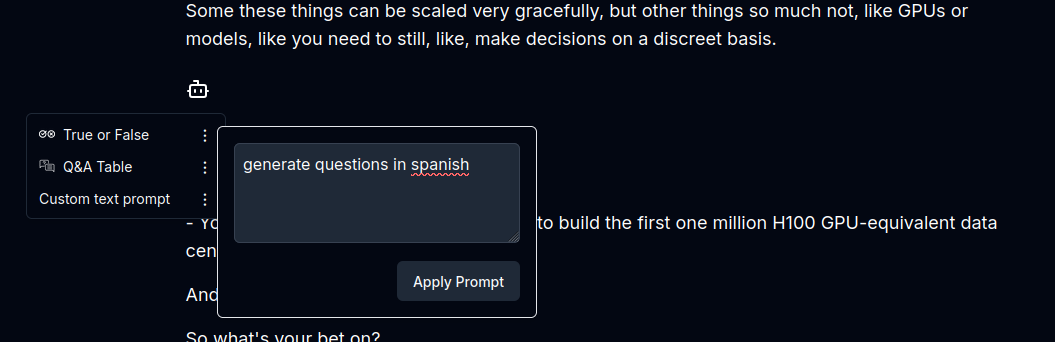
\includegraphics[width=\textwidth,height=0.45\textheight,keepaspectratio]{exemplo-slides/graphics/images/quizzes/customizar-prompt.png}
\caption{Popover para customização do prompt utilizado na geração de questões}
\label{fig:custom_prompt}
\end{figure}

Este campo permite personalizar o comportamento do modelo. Após inserir o prompt personalizado e confirmar, o sistema gera as questões seguindo as diretrizes especificadas.

A Figura \ref{fig:spanish_questions} demonstra um exemplo prático desta funcionalidade, onde o usuário solicitou que as questões fossem geradas em espanhol. 

\begin{figure}[H]
\centering
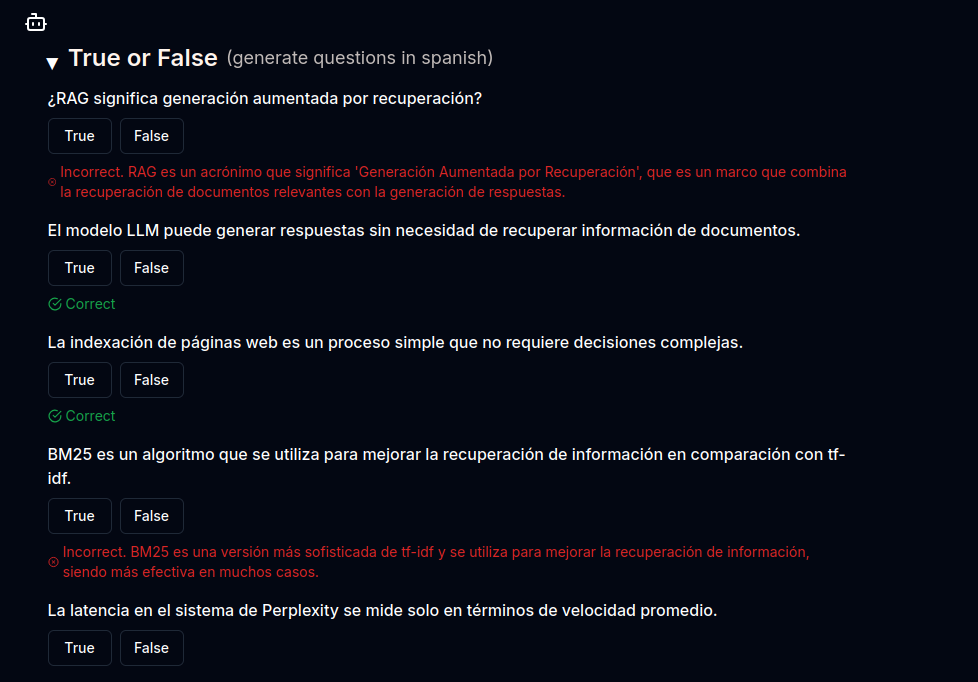
\includegraphics[width=\textwidth,height=0.45\textheight,keepaspectratio]{exemplo-slides/graphics/images/quizzes/generated-spanish-questions.png}
\caption{Questões de Verdadeiro ou Falso geradas em espanhol após customização do prompt}
\label{fig:spanish_questions}
\end{figure}

A exposição do prompt ao usuário traz benefícios significativos ao processo de aprendizagem. Esta transparência permite adaptações para diferentes estilos de aprendizagem e níveis de conhecimento. Os usuários podem experimentar diferentes abordagens e refinar suas instruções para obter resultados mais alinhados com suas necessidades específicas.


\section{Bate-Papo com Vídeo}

O componente de bate-papo com vídeo permite aos usuários fazer perguntas e obter respostas contextualizadas sobre o conteúdo dos vídeos. Esta funcionalidade transforma a experiência de assistir vídeos ao possibilitar interações diretas com o material apresentado.

\begin{figure}[H]
  \centering
  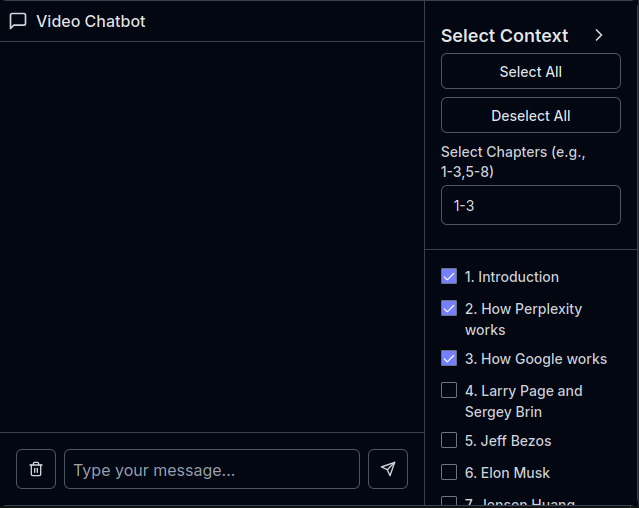
\includegraphics[width=\textwidth,height=0.45\textheight,keepaspectratio]{exemplo-slides/graphics/images/video-chatbot.png}
  \caption{Interface do componente de bate-papo com vídeo, mostrando painel de seleção de contexto e área de conversação}
  \label{fig:video_chatbot}
\end{figure}

\subsection{Interface do Usuário}

A interface do bate-papo é composta por dois elementos principais:

\begin{itemize}
    
    
    \item \textbf{Painel de Seleção de Contexto}: Um painel expansível à direita permite aos usuários escolher quais partes do vídeo são relevantes para suas consultas. Este componente oferece duas modalidades de seleção: checkboxes individuais para cada capítulo e entrada textual com sintaxe simplificada (por exemplo, "1-3,5" para selecionar os capítulos 1, 2, 3 e 5).
    
    \item \textbf{Área de Conversação}: Abaixo do player, a área de chat apresenta as mensagens trocadas entre o usuário e o assistente, com suporte a formatação e indicadores de processamento.
\end{itemize}

Um elemento importante da interface é o botão de exclusão de mensagens, que permite ao usuário limpar todo o histórico de conversa e o contexto selecionado, possibilitando um novo início de interação.

\subsection{Gerenciamento de Contexto}

O sistema implementa duas estratégias principais para seleção de contexto:

\begin{itemize}
    \item \textbf{Contexto com Transcrição na Íntegra}: Quando o vídeo não possui capítulos definidos, o sistema utiliza a transcrição completa como contexto, aplicando truncamento quando necessário.
    
    \item \textbf{Contexto com Transcrição Dividida em Capítulos}: Quando disponíveis, os capítulos permitem uma seleção mais granular, possibilitando ao usuário focar suas consultas em seções específicas do vídeo.
\end{itemize}

Para vídeos extensos sem capítulos, o sistema notifica o usuário sobre a necessidade de truncar a transcrição e sugere a geração de capítulos como alternativa. Quando o contexto selecionado é muito grande, o sistema faz ajustes e informa o usuário através de notificações.

\subsection{Benefícios e Características}

O sistema de bate-papo oferece respostas contextualizadas sobre o conteúdo do vídeo e mantém a coerência conversacional durante a interação. A interface responsiva e o gerenciamento de contexto proporcionam uma experiência prática para análise e discussão do conteúdo em vídeo.

Entre os principais benefícios para o usuário estão:

\begin{itemize}
    \item \textbf{Acesso não-linear ao conteúdo}: Possibilidade de explorar partes específicas do vídeo sem assistir à sequência completa
    \item \textbf{Extração de informações}: Obtenção de respostas específicas sem necessidade de assistir ou rever o vídeo inteiro
    \item \textbf{Personalização da experiência}: Foco em áreas de interesse particular
    \item \textbf{Aprofundamento do entendimento}: Capacidade de fazer perguntas para esclarecer conceitos
\end{itemize}

O sistema transforma a experiência de assistir vídeos ao permitir que os usuários interajam diretamente com o conteúdo através de perguntas e respostas contextualizadas.



\section{Discussão}

Este capítulo apresentou a implementação do VideoLearnAI e as decisões técnicas que moldaram seu desenvolvimento. O projeto enfrentou diversos desafios que exigiram adaptações e mudanças de abordagem ao longo do processo.

Na melhoria de legibilidade das legendas, a tentativa inicial de utilizar LLMs apresentou inconsistências nos resultados, alto custo computacional e tempos de resposta inaceitáveis. A migração para o modelo especializado SaT, executado em infraestrutura serverless GPU, tornou o processo muito mais rápido e confiável, com a vantagem adicional de não alterar o conteúdo original do texto, apenas melhorando sua estruturação.

Para a geração de capítulos, a abordagem inicial de solicitar ao LLM a identificação direta de timestamps mostrou-se imprecisa, pois os modelos de linguagem têm dificuldade em lidar com informações temporais específicas. A solução adotada dividiu o problema em duas etapas: segmentação prévia da transcrição em parágrafos numerados com timestamps associados, seguida pela identificação semântica das transições temáticas pelo LLM, que apenas indicava os números dos parágrafos onde ocorriam mudanças de tópico. Uma lógica posterior recolocava os timestamps corretos com base nos números dos parágrafos identificados. Esta decomposição do problema resultou em capítulos mais coerentes e precisos temporalmente.

Na transcrição de áudio, a migração do Whisper para o Deepgram eliminou a necessidade de segmentação de arquivos longos e reduziu drasticamente o tempo de processamento, melhorando significativamente a experiência do usuário. O Deepgram oferece vantagens adicionais como timestamps no nível da palavra, capacidade de diarização (identificação de diferentes falantes) e um modelo de negócios que disponibiliza créditos gratuitos para desenvolvimento, tornando-o uma escolha mais viável para a plataforma.

Para os quizzes interativos, a decisão de expor os prompts ao usuário final, permitindo personalização, equilibrou simplicidade e flexibilidade, beneficiando tanto usuários iniciantes quanto avançados. O uso de function calling garantiu saídas estruturadas e compatíveis com as interfaces gráficas.

No sistema de bate-papo, a seleção manual de contexto baseada em capítulos foi inicialmente preferida a abordagens mais complexas como RAG (Retrieval-Augmented Generation), priorizando controle do usuário e simplicidade de implementação na fase inicial do projeto. 










\chapter{CONCLUSÃO}

O desenvolvimento do VideoLearnAI demonstrou o potencial significativo da integração entre modelos de linguagem natural e tecnologias web modernas para criar experiências educacionais mais efetivas. A plataforma conseguiu transformar o consumo passivo de vídeos em um processo de aprendizagem ativa, oferecendo ferramentas que promovem maior engajamento e compreensão do conteúdo.

\section{Objetivos Alcançados}

Os objetivos inicialmente propostos foram alcançados através da implementação bem-sucedida das cinco funcionalidades principais:

\begin{enumerate}
    \item \textbf{Melhoria da Legibilidade das Legendas:} A implementação do modelo SAT (Segment Any Text) proporcionou uma solução eficiente e precisa para a segmentação de texto, superando as limitações encontradas na abordagem inicial com LLMs. Esta funcionalidade demonstrou ser fundamental para melhorar a experiência de leitura e compreensão do conteúdo.

    \item \textbf{Geração de Capítulos:} O sistema de geração automática de capítulos, combinando segmentação de texto com análise por LLMs, mostrou-se eficaz na organização estruturada do conteúdo, facilitando a navegação e o acesso a informações específicas.

    \item \textbf{Legendas de maior qualidade:} A geração de legendas com o serviço Deepgram ao invés das legendas geradas automaticamente pelo youtube, resultou em um processo mais eficiente e preciso de transcrição, com benefícios adicionais como marcação temporal no nível da palavra e capacidade de diarização dos locutores.

    \item \textbf{Quizzes Interativos:} Superando as limitações do consumo passivo de vídeo, os questionários interativos com feedback em tempo real promovem engajamento ativo através de exercícios práticos e reflexivos, maximizando a absorção do conteúdo.

    \item \textbf{Bate-Papo Contextual:} O sistema de chat contextualizado proporcionou uma forma natural e eficiente de interação com o conteúdo do vídeo, com gerenciamento adequado de contexto, transparente para o usuário.

    \item \textbf{Sistema de Salvamento de Progresso:} Foi implementado um mecanismo que permite aos usuários salvar seu progresso de estudo. Esta funcionalidade possibilita que os usuários retomem seus estudos exatamente de onde pararam, promovendo continuidade no processo de aprendizagem.
  \end{enumerate}

\section{Trabalhos Futuros}

Após a implementação inicial do VideoLearnAI, ficou evidente que além das funcionalidades básicas já desenvolvidas, existem melhorias possíveis que podem enriquecer gradualmente a experiência dos usuários. A seguir, apresento algumas propostas viáveis para o aprimoramento contínuo da plataforma

Uma evolução natural seria aproveitar plenamente os recursos já disponíveis no serviço Deepgram, especificamente a funcionalidade de diarização que já está incluída na API utilizada. A integração desta capacidade permitiria identificar e diferenciar múltiplos falantes nas transcrições, enriquecendo substancialmente a experiência do usuário através de elementos visuais distintivos como legendas coloridas ou avatares para cada interlocutor. Esta implementação não exigiria mudanças significativas na infraestrutura existente, apenas o processamento adicional dos metadados de diarização já fornecidos pelo Deepgram. Além de melhorar a legibilidade, esta funcionalidade forneceria contexto adicional valioso para o sistema de chat e geração de quizzes, permitindo análises mais granulares do conteúdo e facilitando a compreensão de debates e discussões em grupo.

Um aprimoramento significativo para a legibilidade das legendas seria a implementação de modelos especializados em pontuação automática, complementando o atual sistema de segmentação de parágrafos. A integração destes modelos permitiria a adição precisa de sinais de pontuação, aproximando a transcrição de um texto natural e fluido. 

A evolução do sistema de quizzes para incorporar princípios de repetição espaçada representa outra frente promissora. Esta abordagem, fundamentada em pesquisas sobre memória e retenção de conhecimento, programaria revisões estratégicas do conteúdo em intervalos crescentes, maximizando a retenção de longo prazo. A implementação poderia incluir notificações personalizadas para revisão de conceitos específicos e adaptação dinâmica da dificuldade das questões com base no histórico de desempenho do usuário, criando um ciclo de aprendizado verdadeiramente adaptativo.

Para o componente de bate-papo, a integração de um sistema RAG (Retrieval-Augmented Generation) agêntico representaria um salto qualitativo significativo. Esta evolução permitiria que o sistema não apenas respondesse a perguntas com base no contexto selecionado, mas também navegasse inteligentemente por todo o conteúdo do vídeo, recuperando informações relevantes de forma autônoma. Um sistema RAG agêntico poderia realizar análises comparativas entre diferentes seções do vídeo, identificar contradições ou complementaridades no discurso e até mesmo buscar informações em fontes externas quando apropriado, tudo mantendo uma interação natural e contextualizada com o usuário.

A dimensão social da aprendizagem poderia ser explorada através da implementação de elementos de gamificação centrados na competição saudável. Um sistema de ranking por vídeo permitiria aos usuários comparar seu desempenho nos quizzes com outros estudantes, estimulando maior engajamento com o conteúdo. Esta funcionalidade poderia ser expandida para incluir badges por conquistas específicas, como completar todos os quizzes de um vídeo ou manter uma sequência de respostas corretas. Tais elementos de gamificação não apenas tornariam a experiência mais envolvente, mas também forneceriam motivação adicional para os usuários revisitarem conteúdos e aprimorarem seu entendimento, transformando o processo de aprendizagem em uma atividade mais dinâmica e recompensadora.

Por fim, a internacionalização da plataforma representa uma oportunidade significativa de expansão. A implementação incluiria a tradução da interface do usuário para múltiplos idiomas e a integração com serviços de tradução como o \textit{DeepL}\footnote{\url{https://www.deepl.com/pt-BR/translator}} para converter automaticamente as legendas dos vídeos. Esta abordagem simplificada removeria barreiras linguísticas ao conhecimento, permitindo que usuários acessem conteúdo educacional independentemente do idioma original, sem necessidade de implementações complexas adicionais.

Estas direções de desenvolvimento, embora ambiciosas, são tecnicamente viáveis e alinhadas com a visão original do VideoLearnAI: transformar o consumo passivo de vídeos em experiências de aprendizagem ativas, personalizadas e eficazes. 






% Bibliografia http://liinwww.ira.uka.de/bibliography/index.html um
% site que cataloga no formato bibtex a bibliografia em computacao
% \bibliography{nomedoarquivo.bib} (sem extensao)
% \bibliographystyle{formato.bst} (sem extensao)







\bibliographystyle{abnt}
\bibliography{bibliografia} 












\end{document}


